
\documentclass[12pt,a4paper,twoside]{book}

%% general usepackage stuff
\usepackage{times}
\usepackage{mathptmx}
\usepackage{booktabs}
\usepackage{graphicx}
\usepackage{titlesec}
\usepackage{amssymb}
\usepackage[british,UKenglish,USenglish,english,american]{babel}
\usepackage{color}

%% labels and page stuff
\renewcommand{\labelitemi}{$\diamond$}
\renewcommand{\labelitemii}{$\circ$}

\setcounter{secnumdepth}{3}

%\setlength{\oddsidemargin}{-0.5cm}
%\setlength{\evensidemargin}{-0.5cm}

\setlength{\oddsidemargin}{4.58mm}%final
\setlength{\evensidemargin}{-4.92mm}%final


\setlength{\textwidth}{15.95cm}%final
\setlength{\textheight}{23.5cm}
\setlength{\voffset}{-1.45cm} %


%% todo
\newcommand{\todo}[1]{\textcolor{red}{[todo: }#1\textcolor{red}{]}}
\newcommand{\todoh}[1]{} 
\newcommand{\done}[1]{} 

%% smallerText
\newcommand{\smallerTextSize}{10}
\newcommand{\smallerTextSkip}{12}
\newcommand{\smallerBegin}{\fontsize{\smallerTextSize}{\smallerTextSkip}\selectfont}
\newcommand{\smallerEnd}{\normalsize}
\newcommand{\smaller}[1]{\smallerBegin #1\smallerEnd}

%%reference to defintion
\newcommand{\defref}[1]{\ref{#1} on page \pageref{#1}}

%% special, short for shell
\newcommand{\shl}[1]{\sf \small #1\rm\normalsize}

%% indentation in tables
\newcommand{\tabind}[1]{\rule{#1mm}{0cm}}

%% smaller in captions
\newcommand{\captionfonts}{\smallerBegin}
                                                                                                                                                                              
\makeatletter  % Allow the use of @ in command names
\long\def\@makecaption#1#2{%
  \vskip\abovecaptionskip
  \sbox\@tempboxa{{\captionfonts #1: #2}}%
  \ifdim \wd\@tempboxa >\hsize
    {\captionfonts #1: #2\par}
  \else
    \hbox to\hsize{\hfil\box\@tempboxa\hfil}%
  \fi
  \vskip\belowcaptionskip}
\makeatother   % Cancel the effect of \makeatletter

%% clear page before new chapter
\makeatletter
\def\cleardoublepage{\clearpage\if@twoside \ifodd\c@page\else
\hbox{}
\vspace*{\fill}
\begin{center}
%This page intentionally contains only this sentence.
\end{center}
\vspace{\fill}
\thispagestyle{empty}
\newpage
\if@twocolumn\hbox{}\newpage\fi\fi\fi}
\makeatother

%% abbreviations
\usepackage{nomencl}
\let\abbrev\nomenclature
\renewcommand{\nomname}{List of Abbreviations}
\setlength{\nomlabelwidth}{.25\hsize}
\renewcommand{\nomlabel}[1]{#1 \dotfill}
\setlength{\nomitemsep}{-\parsep}
\makenomenclature
\newcommand{\Listofabbrev}{
\printnomenclature
\newpage
}

%% chapter title formatting
\titleformat{\chapter}[display]{ \raggedleft }{\fontsize{52}{63}\selectfont \bf \thechapter }{0.2cm}{\fontsize{32}{38.7}\selectfont  }[]

%% haeder formatting
\renewcommand{\chaptermark}[1]{%
\markboth{\chaptername
\ \thechapter.\ #1}{}}
\renewcommand{\sectionmark}[1]{\markright{\thesection.\ #1}}
\usepackage{fancyhdr}
\pagestyle{fancy}
\fancyhf[LEH,ROH]{\thepage}
\fancyhf[REH]{\smaller{\nouppercase{\leftmark}}}
\fancyhf[LOH]{\smaller{\it \nouppercase{\rightmark}}}
\fancyhf[COF]{\rule{0.2cm}{0.0cm}}
\fancyhf[CEF]{\rule{0.2cm}{0.0cm}}
\renewcommand{\headrulewidth}{0pt}

%% macro for figures

%\newcommand{\printlabel}{}
%\newcommand{\abcdef}[1]{\tiny #1 \normalsize}

		%% arguments: graphics file, label, caption, smallcaption
\newcommand{\insertFigure}[4]{\begin{figure}[top] \smallerBegin \centering \includegraphics{#1}  \\  \caption{\label{#2}\smallerBegin #3 \footnotesize{#4}  \smallerEnd }  
\end{figure}	}
%% macro for figures with short caption
		%% arguments: graphics file, label, caption, smallcaption, shortcaption
\newcommand{\insertFigureShort}[5]{\begin{figure}[top] \smallerBegin \centering \includegraphics{#1} \label{#2} \\ \caption[#5]{\smallerBegin #3 \footnotesize{#4} \smallerEnd } 
\end{figure}	}
%\renewcommand{\topfraction}{1}

\newcommand{\spaceafterpar}{\vspace{14.48pt}}

\renewcommand{\floatpagefraction}{.75} % vorher: .5
\renewcommand{\textfraction}{.1}       % vorher: .2
\renewcommand{\topfraction}{.8}        % vorher: .7
\renewcommand{\bottomfraction}{.5} 
\setcounter{topnumber}{3}              % vorher: 2
\setcounter{bottomnumber}{2}           % vorher: 1
\setcounter{totalnumber}{5}            % vorher: 3
%from: http://www.matthiaspospiech.de/latex/vorlagen/allgemein/preambel/9/

%macros for tables
    %% arguments: columns
\newcommand{\tableBegin}[1]{\begin{table}[top] \begin{center} \smallerBegin \begin{tabular}{#1}\\ \toprule}
		%% arguemtns: caption, label
\newcommand{\tableEnd}[2]{\bottomrule \end{tabular} \smallerEnd \end{center} \caption{#1} \label{#2}	\end{table}}

%% shortcuts
\newcommand{\emit}[1]{\item \emph{#1}:}
\newcommand{\firstappear}[2]{\emph{#1} (#2) \abbrev{#2}{#1}}

\hyphenation{or-gan-izing}

%% definitions

\newtheorem{definition}{Definition}

%% examples
\newcommand{\exampleBeginText}[1]{\paragraph{#1}}
\newcommand{\exampleEnd}{\vspace{6mm}}
\newcommand{\exampleBegin}{\exampleBeginText{Example}}


% Front Matter

\newcommand{\titleLineOne}{Detection of Higher-Level Concepts}
\newcommand{\titleLineTwo}{ in Highly-Linked Big Data}
\newcommand{\titleLineThree}{}
\newcommand{\documentdate}{December 22, 2015}
\newcommand{\studentname}{Max Mustermann}
\newcommand{\abstracttext}{Short version of the thesis in 250 words.}
\newcommand{\acktext}{First of all, I would like to...}

\begin{document} 

%\thispagestyle{empty}
\rule{0cm}{2cm}

\fontsize{19.83}{26.45} \selectfont 
\noindent \textbf{\titleLineOne} \vspace{0.2cm}
\\\textbf{\titleLineTwo}\vspace{0.2cm}
\\\textbf{\titleLineThree}
\normalsize

\newpage
\thispagestyle{empty}
\rule{0cm}{2cm}
\newpage

\thispagestyle{empty}
\rule{0cm}{1.5cm}

\fontsize{26.44}{32} \selectfont 
\noindent \textbf{\titleLineOne} \vspace{0.2cm}
\\\textbf{\titleLineTwo}\vspace{0.2cm}
\\\textbf{\titleLineThree}
\normalsize

%\noindent ---Draft--- \vspace{-0.75cm}


\vspace{1.5cm}
 
\noindent \textbf{\studentname}

\vspace{-0.25cm}
\vspace{7cm}
%\vspace{10cm}

\noindent A thesis submitted to the 
\\\textbf{Faculty of Electrical Engineering and Computer Science
} 
\\of the 
\\\textbf{Technical University of Berlin} 
\\in partial fulfillment of the requirements for the degree 
\\\textbf{Master of Computer Science}

\vspace{-0.5cm}
 
\noindent Berlin, Germany\\ 
\documentdate\\

\vspace{-0.83cm}
%\vspace{1cm}

\noindent 
\includegraphics[width=30mm,angle=0]{graphics/tu_logo}

\rule{0cm}{20cm}

\noindent Main supervisor: 

\noindent Prof. Dr. habil. Odej Kao, Technical University of Berlin

%\noindent Date of public examination: November 20, 2009
\thispagestyle{empty}


\chapter*{Abstract}

\abstracttext

\thispagestyle{empty}
\newpage
\vspace*{3cm}
\thispagestyle{empty}

\chapter*{Acknowledgements}

\acktext


\thispagestyle{empty}
\newpage
\vspace*{3cm}
\thispagestyle{empty}

%% indices


%\thispagestyle{empty}
\pagenumbering{roman}\setcounter{page}{8}
\tableofcontents

%\thispagestyle{empty}
\newpage


\listoffigures
\listoftables
\Listofabbrev
\newpage
\thispagestyle{empty}
\newpage
\vspace*{3cm}
\thispagestyle{empty} \newpage
\pagenumbering{arabic}\setcounter{page}{1}

% Body Matter (use input to add chapters)

%\chapter{Introduction}
%All the reader needs to know to get introduced to the topic. What is this thesis about? %Why is it interesting? Give the reader a brief idea of the structure of the thesis. One %page.
\chapter{Background}
% The goal of a detection system is to group together stories that discuss the same event.
%Necessary background for topic, in order to understand the problem, motivation, related %work and contribution. Approximately 10 pages.
In this section, we will give an overview of the needed theoretical background to understand this thesis.
\section{Big Data}
Today’s society is witnessing an exponential increase in the amount of generated data. For instance, retailers, social medias, organizations in financial and healthcare sectors are all generating large volumes of data that need to be collected and analyzed to make the appropriate decisions. In this section, we will give an overview of Big Data characteristics and analytics methods.
 \subsection{Definition}
The term Big Data applies to information that could not be processed using traditional processes or tools \cite{a:IBM}.
For instance, Edd Dumbill defined Big Data according to its processing aspect as follows:\\
		"Big data is data that exceeds the processing capacity of conventional database systems. The data is too big,   		moves too fast, or doesn’t fit the structures of your database architectures" \cite{a:def1}.\\
Another definition of Big Data based on the three dimensions: \textit{Volume}, \textit{Variety} and \textit{Velocity} has emerged. For instance, Gartner Inc. defined Big Data as follows: \\
		"Big data is high-volume, high-velocity and/or high-variety information assets that demand cost-effective, innovative forms of information processing that enable enhanced insight, decision making, and process automation." \cite{a:gartner}.\\
	Some other definitions add the term \textit{Veracity} to the 3 V model to characterize Big Data \cite{a:veracity}.\\
	In the remainder of this section, we will go through each of these Big Data aspects. 
 	\begin{enumerate}
		\item Volume: \\ refers to the quantity of data which is reported in multiple terabytes and petabytes.  
	   	\item Variety: \\ refers to the diverse types of data which can be:\\
		structured data refers to information with a high degree of organization, such that inclusion in a relational database is seamless and readily searchable by simple, straightforward search engine algorithms or other search operations; whereas unstructured data is essentially the opposite. The lack of structure makes compilation a time and energy-consuming task. It would be beneficial to a company across all business strata to find a mechanism of data analysis to reduce the costs unstructured data adds to the organization. \cite{a:https://brightplanet.com/2012/06/structured-vs-unstructured-data/}
	   	\begin{description}
		\item[-] structured data: refers to highly organized data that can be easily stored in a relational database. \cite{a:https://brightplanet.com/2012/06/structured-vs-unstructured-data/} \\
		\item[-] unstructured data:.
refers to data with no structural organization such as texts, images, audios and videos. \cite{a:https://jeremyronk.wordpress.com/2014/09/01/structured-semi-structured-and-unstructured-data/}\\
		\item[-] semi-structured data: refers to data that have some organizational properties, after some process it could be stored in a relational database. Examples of this type of data include XML and JSON documents. NoSQL databases are considered as semi structured. \cite{a:https://brightplanet.com/2012/06/structured-vs-unstructured-data/} 
		\end{description}
			
		\item Velocity:\\ it refers to the rate at which data are generated and the
speed at which it should be analyzed and acted upon \cite{a:Beyond  the  hype}.
	    \item Veracity: \\ it refers to the biases, noise and abnormality in data. 	 
	\end{enumerate}	

\subsection{Big Data analytics}
Big Data analytics aims to obtain meaningful results from big data by providing algorithms that include statistical models, machine learning, text analytics  and other advanced data-mining techniques.
\subsubsection{Text analytics}
Text analytics deals with analyzing unstructured text, extracting relevant information, and transforming it into structured information that can then be leveraged in various ways. It uses techniques from Natural Language Processing (NLP), knowledge discovery, data mining, information retrieval, and statistics..
\begin{enumerate}
\item  Natural Language Processing: \\
 NLP is a complex field that aims  to develop tools and techniques to make computer systems understand and manipulate natural languages to perform the desired tasks. It generally makes use of linguistic concepts such as grammatical structures and parts of speech to determine who did what to whom, when, where, how, and why \cite{a:BigData} \cite{a:NLP}.\\
NLP performs analysis on text at different levels:
\begin{itemize}
\item Lexical/morphological:  deals with understanding the meaning of words and parts of speech (such as noun, verb, adjective) in the context of the text provided. The lexical analyzer connects each word with its corresponding label in a dictionary. The morphological analyzer identifies words or phrases in one sentence and marks each word with a token symbol. The identified tokens are classified according to their grammatical class \cite{a:analyzer http://www.sbmac.org.br/dincon/trabalhos/PDF/statistics/68066.pdf}.
\item Syntactic analysis aims to check that a sentence is well formed and to break it up into a structure that shows
the syntactic relationships between the different words. This is done using a dictionary of word definitions and a set of grammar rules \cite{a:https://www.scm.tees.ac.uk/isg/aia/nlp/NLP-overview.pdf}.
\item Semantic analysis determines the possible meanings of a sentence. This can include examining word order and sentence structure and disambiguating words by relating the syntax found in the phrases, sentences, and paragraphs.
\item Discourse-level analysis attempts to determine the meaning of text beyond the sentence level \cite{a:BigData}.
\end{itemize}
These techniques are generally combined with other statistical or linguistic techniques to automate the tagging and markup of text documents to extract the following informations \cite{a:BigData}:
\begin{itemize}
\item  Terms: these are the keywords.
\item  Entities: or named entities, these are specific examples of
abstractions (tangible or intangible). Examples are names of persons,
names of companies, geographical locations, contact information, dates,
times, currencies, titles and positions, and so on. 
\item  Facts: Also called relationships. They indicate the who/what/where relationships
between two entities. 
\item  Events: events usually contain a time dimension and often cause facts to
change. 
\item  Concepts: These are sets of words and phrases that indicate a particular
idea or topic with which the user is concerned. This can be done
manually or by using statistical, rule-based, or hybrid approaches to
categorization. Concepts can be defined by users to suit their particular needs.
\item  Sentiments: Sentiment analysis is used to identify viewpoints or emotions
in the underlying text. Some techniques do this by classifying text as, for example, subjective (opinion) or objective (fact), using machine learning or NLP techniques.
\end{itemize}
\end{enumerate}
\subsection{Big Data Processing Frameworks}
The MapReduce \cite{a:mapR} framework stayed for a long time the reference standard for big data processing,
however, it is not suited for wide range of applications, such as
real time and machine learning. In the last years, a variety of
big data processing engines that tackel its shortcomings were
developped.
MapReduce revolutionized computation over huge data sets by
offering a simple model for writing programs that could execute in parallel across hundreds to thousands of machines. 
\subsubsection{The difference between batch and stream processing}
\begin{itemize}
\item[-] batch processing: refers to a type of engines that process finite “batch” data sets as bounded data \cite{a:Akidu}. Batch processing systems are based on the ETL technology. ETL tools are used to transform the data into the format required by the data warehouse, which provide business users with a way to consolidate information across disparate sources (such as enterprise resource planning [ERP] and customer relationship management [CRM]) to analyze and report on data relevant to their specific business focus, by performing the following functions:
\begin{itemize}
\item [-] Extract: Read data from the source database.
\item [-] Transform:Convert the format of the extracted data so that it conforms to the requirements of the target database. Transformation is done by  using rules or merging data with other data.
\item [-] Load: Write data to the target database.
\end{itemize}
 ETL tools extracted the data to an intermediary location to perform the transformation before loading the 
data to the data warehouse.
Data warehouses provide business users with a way to consolidate information across disparate sources (such as enterprise resource planning [ERP] 
and customer relationship management [CRM]) to analyze and report on 
data relevant to their specific business focus.
\item[-] stream processing:
According to \cite{a:amazon}, streaming data is data that is generated continuously by thousands of data sources, which typically send in the data records simultaneously, and in small sizes (order of Kilobytes). It can also be described as infinite or unbounded data \cite{a:Akidu}.
Tylor Akidu, an engineer in the Google Cloud DataFlow team, defined stream processing as data processing engine that is designed with infinite data sets in mind \cite{a:Akidu}. For instance, an online gaming company that collects streaming data about player-game interactions, and feeds the data into its gaming platform. It then analyzes the data in real-time, offers incentives and dynamic experiences to engage its players.
\end{itemize}
				\begin{figure}[h!]
					\centering
					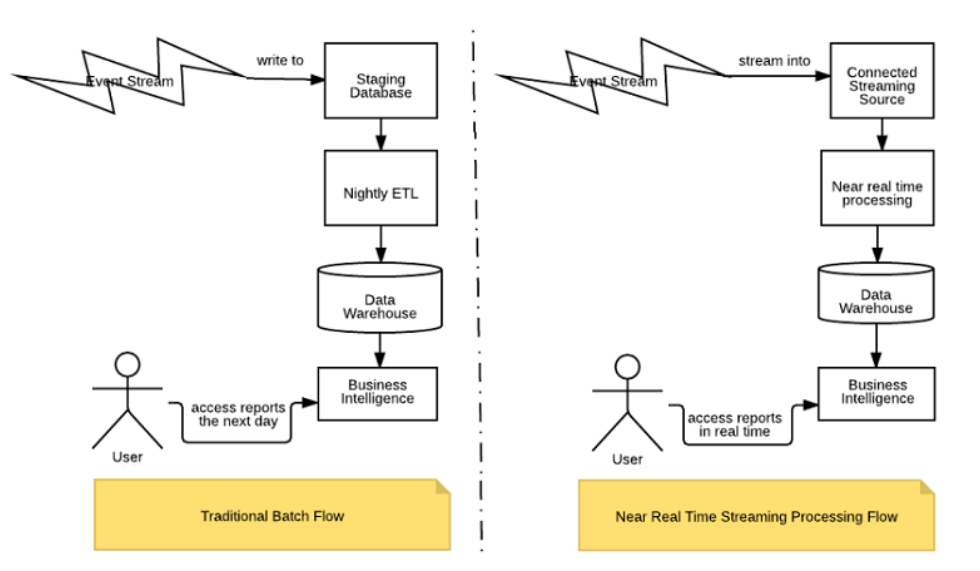
\includegraphics[scale=0.5]{graphics/BatchStream.PNG} 
					\caption{ Comparison between batch and stream processing dataflows \cite{a:Flink}} \label{flink} 
				\end{figure}
In a batch-processing scenario, the transactions databases collect event data during the day, which is bulk loaded to a staging database at night. A large ETL process then executes to produce aggregations on this data and store these results to the data warehouse. The Business Intelligence applications then present the reports based on  these aggregates to the business users the following day. Users have to wait an entire day to get insights into business 
operations.\\
Streaming systems operate differently. The transactions database will stream the logs in near real-time which are processed by a streaming system which will produce aggregations within intervals such as time. For example, calculate aggregates like total sales by region for every 5-minute interval. We will soon see that other types of intervals 
are also possible in Flink. These aggregates will be stored in the Data Warehouse which provide a more real-time insight into business operations to the business users. The intervals should not be too small (ex. 5-seconds) because Data Warehouses are typically designed for optimal reads (lots of indexes) which will slow down the writing of the granular aggregates and cause the overall system to have bottlenecks.				

\subsubsection{Apache Flink}
Apache Flink is an open source platform that uses a common runtime for scalable batch and stream data processing. Flink's stack includes the DataStream and the DataSet APIs for creating stream processing and batch processing applications respectively. It also bundles libraries for domain-specific use cases such as Machine learning and graph analytics. A Flink Program can be easily deployed according to three different modes: locally, on a existing YARN or a Standalone cluster or on existing clusters in the cloud.
\begin{itemize}
\item[-] Local Mode: ... \\
%Local mode is a pseudo distributed mode which runs all the daemons in the single jvm. It uses AKKA framework for %parallel processing which underneath uses multiple threads.
\item[-] Standalone Cluster Mode: ...\\
%In this setup, different daemons runs on different jvms on a single machine or multiple machines. This mode often %used when we want to run only Flink in our infrastructure.
\item[-]YARN:... \\
%This mode makes flink run on YARN cluster management. This mode often used when we want to run flink on our existing hadoop clusters.
\end{itemize}
				\begin{figure}[h!]
					\centering
					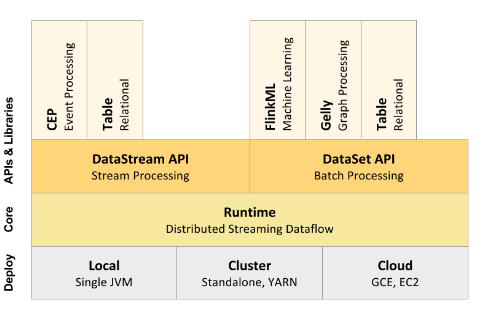
\includegraphics[scale=0.7]{graphics/Flink-Stack.PNG} 
					\caption{ Flink Stack \cite{a:BigData}} \label{flink} 
				\end{figure}


\textbf{- Flink's architecture overview:}\\
After a Flink program is submitted, three processes are put into place to compile it:
\begin{itemize}
\item[-]  A \textbf{Client} is created that performs the pre-processing and transforms the program into an optimized JobGraph, a generic parallel data flow with arbitrary tasks that consume and produce data streams, and sends it to  the JobManager. After that, it can disconnect, or stay connected to receive progress reports.The client program runs either as part of the Java/Scala program that triggers the execution, or in the command line process. 
\item[-] 	The \textbf{JobManagers} (also called masters) they ensure the program parallelization by coordinating the distributed execution of the execution Graph. They schedule tasks by assigning tasks to Task Managers, they also perform other tasks such as checkpoints coordination and recovery on failures coordination.\\
A Flink program uses at least one Job Manager. To ensure high-availability, a setup would use multiple JobManagers, with one leader and the other JobManagers as standby .
\item[-] 	The \textbf{TaskManagers} (also called workers) execute the tasks (or more specifically, the subtasks) of a dataflow, and buffer and exchange the data streams.
Operations are split up into tasks depending on the specified parallelism § Each parallel instance of an operation runs in a separate task slot § The scheduler may run several tasks from different operators in one task slot
There must always be at least one TaskManager. \\
 TaskManagers connect to JobManagers, announcing themselves as available, and are assigned work.\\
\end{itemize} 
			\begin{figure}[h!]
					\centering
					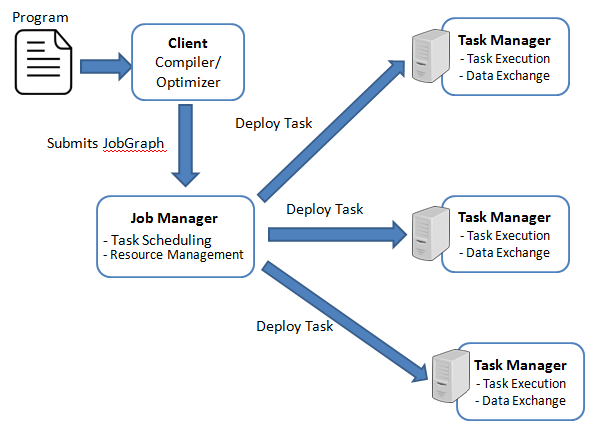
\includegraphics[scale=0.7]{graphics/compilation.PNG} 
					\caption{Flink Architecture Overview} \label{archi} 
			\end{figure}
				

\textbf{- Apache Flink Programming Model:}
\begin{itemize}
\item[-] Program Dataflow:\\
 
 A Flink program can be viewed as a streaming dataflow that takes the data streams from a source, performs transformation operations on it and stores the resulting streams in a sink.
Programs in Flink are inherently parallel and distributed.
 				\begin{figure}[h!]
					\centering
					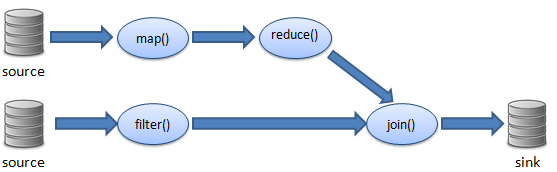
\includegraphics[scale=0.7]{graphics/concepts.PNG} 
					\caption{Flink Streaming dataflow} \label{dataflow} 
				\end{figure}
Data sources create the initial Datasets, from Text or CSV files or from Java collections. \\
					Data sinks store the returned values after the transformations in a Dataset.\\
					Data transformations transform one or more DataSets into a new DataSet. Programs can combine multiple transformations into sophisticated assemblies. Some common transformations and their definitions according to Flink's documentation \cite{transf} include:
\begin{itemize}
\item[-] Map(): \\	
Takes one element and produces one element.
\item[-] Filter(): \\	
Evaluates a boolean function for each element and retains those for which the function returns true.
\item[-] Reduce(): \\	
Combines a group of elements into a single element by repeatedly combining two elements into one. Reduce may be applied on a full data set, or on a grouped data set.
\item[-] Join(): \\	
	Joins two data sets by creating all pairs of elements that are equal on their keys.
	 \end{itemize}
 \item[-]\textbf{ Time:}
Time
When processing data which relate to events in time, there are three inherent domains of time to consider. 
	\begin{itemize}
\item   Event time:\\
 is the time at which the event itself actually occurred, it is usually described by a timestamp attribute in the event data and is assigned by the source of the event. Flink accesses event timestamps via timestamp assigners.
 Once assigned, the event time for a given event never changes.
 
\item 	Ingestion time:\\ 
This is the time the event arrives to the Flink dataflow at the source operator. It is assigned by the Flink system.  Like the event time, it is assigned once and never changes. 

\item	Processing Time:\\
  is the current time according to the system clock at which an event is observed at any given point during processing at each operator that performs a time-based operation. It changes constantly for each event as it arrives for processing at an operator instance.
\end{itemize}

 \item[-] Window: \\
Windowing slices up a dataset into finite chunks for processing as a group, it contains multiple events on which several operation types such as aggregation can be applied on events in a window. Windowing can be applied to both batch and stream processing.\\
In batch processing where bounded data is processed, windowing is an optional concept of semantic usefulness. \\
In stream processing where unbounded data is processed, the windowing concept is crucial for some operations to delineate finite boundaries in most forms of grouping such as aggregation and unnecessary for others such as filtering and mapping.\\
Flink contains two windows types: built-in time and count based windows that can be further subdivided into 
tumbling and sliding windows.
\begin{description}
\item[-] Time-based windows: time windows group stream elements by time. They can be defined as tumbling or sliding. 
\begin{description}
\item[-] Tumbling windows: A tumbling time window collects events for a specific time and applies a function on all events in the window after the time is passed and each event is assigned to one only one window. \\
Let's consider the example of an online gaming application, where a gaming server receives immediately after the completion of an instance of game data streams that contain the player identifier, an event time stamp and the score. let's suppose we want to track the generated events each 5 seconds. Figure \ref{win1} illustrates this example.

				\begin{figure}[h!]
					\centering
					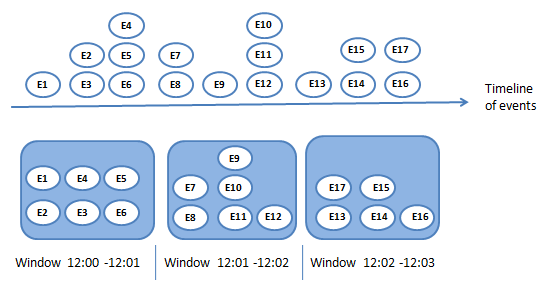
\includegraphics[scale=0.7]{graphics/thumbling.PNG} 
					\caption{ Tumbling windows} \label{win1} 
				\end{figure}
\end{description}

 Time windows can also be sliding.Figure \ref{win2} illustrates a sliding window which is one minute long which slides every 30 seconds.
				\begin{figure}[h!]
					\centering
					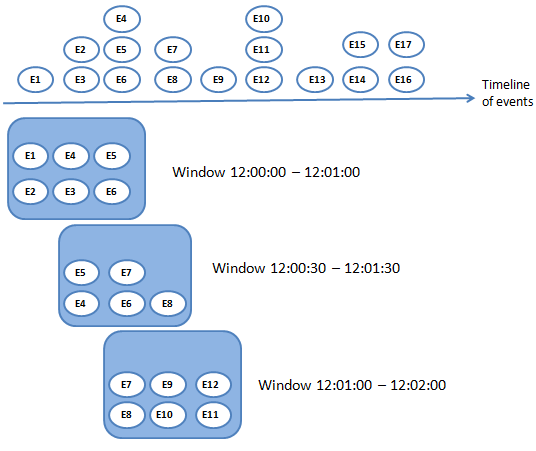
\includegraphics[scale=0.7]{graphics/sliding.PNG} 
					\caption{ Sliding windows} \label{win2} 
				\end{figure}

\item[-] Count-based windows: \\
				in this case, each window is evaluated based on the number of elements it contains. We also distinguish here between tumbling and sliding count based windows. \\
In tumbling count window, the window pane is evaluated when the element count in the pane reaches a pre-defined level, whereas in sliding count windows, the window pane is evaluated based on the number of elements it contains and how much it slides by.
				

\end{description}





\end{itemize}



\subsubsection{Apache Spark}
Apache Spark is an open source framework that combines an engine for distributing programs across clusters of machines with an elegant model for writing programs atop it which was originated at the UC Berkeley AMPLab\cite{a:Spark1}. \\
Figure \ref{stack} depicts the Apache Spark stack components. 
				\begin{figure}[h!]
					\centering
					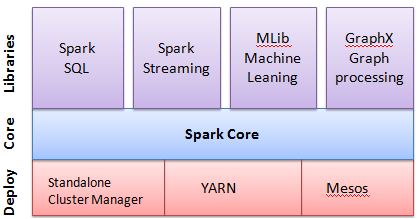
\includegraphics[scale=0.9]{graphics/sparkStack.PNG} 
					\caption{The components of the Spark Stack} \label{stack} 
				\end{figure}

A Spark program follows a master/slave architecture with one central coordinator called driver that launches
various parallel operations on cluster nodes called executors via a cluster manager such as Hadoop YARN or the standalone Hadoop manager. Figure \ref{spark} depicts the components of a distributed Spark application.
				\begin{figure}[h!]
					\centering
					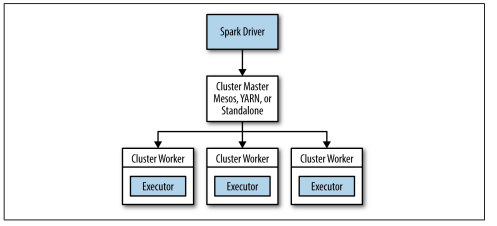
\includegraphics[scale=0.9]{graphics/spark.PNG} 
					\caption{The components of a distributed Spark application\cite{a:Spark2}} \label{spark} 
				\end{figure}
				The Spark engine implicitly creates a logical directed acyclic graph (DAG) of operations and optimizes this graph by rearranging and combining operators where possible. For instance if we suppose that a Spark job contains a map operation followed by a filter operation, the Spark DAG optimizer would rearrange the order of these operators, so that the number of records would be reduced before a map operation takes place \cite{a:Spark2}.\\
When the driver runs, it converts this logical graph into a physical execution plan, where each stage of this plan consists of multiple tasks. The Spark Driver tries to schedule each task in an appropriate Executor.\\ 
				The resilient distributed dataset (RDD)is the Spark’s core abstraction for working with data,  a fault-tolerant collection of elements that can be operated on in parallel \cite{a:Spark3}.
Every Spark program consists of creating some input RDDs from external data and performing operations on those RDDs. The two major types of operations are:
\begin{itemize}
\item \textbf{Transformations:} They take an RDD as an input and produce one or many RDDs. Existing transformations include map(), filter()%, count(), distinct().
\item \textbf{Actions:} They are computations performed on a RDD that return a value. Some supported actions include reduce()%, count(), first(), and foreach().
\end{itemize}
The RDD contents are stored into memory across the cluster nodes, meaning that the future recomputations on an RDD content need not to recompute it or reload it from disk \cite{a:Spark1}.
\subsubsection{Performance comparison between Apache Spark and Apache Flink}
 	Ovidiu-Cristian Marcu et al. provided in \cite{a:comp} a performance comparison between Apache Spark and Apache Flink. The authors performed a series of extensive experiments involving six representative workloads for batch
and iterative processing. \\As for batch workloads, three benchmarks implementing the Word Count\cite{wc}, Grep\cite{wc} and Tera Sort\cite{wc} were selected.\\ As for iterative workloads, three benchmarks evaluating the loop-caching: K-Means, Page Rank\cite{wc} and Connected Components\cite{wc} algorithms were selected.\\ 
For both frameworks, some parameters have influence on some performance metrics such as the overall execution time, scalability and resource consumption. \\ These parameters manage the task parallelism, the
network behavior during the shuffle phase, the memory and the data serialization. 
 For the batch workloads, the goal was to validate strong and weak scalability. For the iterative workloads, the focuse was on scalability, caching and pipelining performance.\\
Two experiment secanrios were conducted, the first scenario consists of having the same dataset size and increasing the number of nodes to characterize the weak scalability, the second scenario consists of having the same the number of nodes and increasing the dataset size to characterize the strong scalability.
\begin{description}
\item[- ] Batch Workload:\\

\begin{tabular}{|l|p{3.5cm}|p{3.5cm}|p{3.5cm}|p{2cm}|}
    \hline
      & \textbf{Word Count} & \textbf{Grep} & \textbf{Tera Sort}\tabularnewline 
    \hline 
      \textbf{Weak Scalability} & both frameworks show a similar performance for a small number of nodes (2 to 8).  
      				   For a larger number (16 and 32), Flink performs slightly better. 
      				  & Spark outperforms Flink, with up to 20\% smaller execution times for large datasets (16 and 						32 nodes).
 						& Flink is performing on average better than Spark, showing smaller execution time. \tabularnewline 
     \hline 
      \textbf{Strong Scalability} & Flink constantly outperforms Spark by 10\%. 
      					 & Spark outperforms Flink  
      					 & Flink’s advantage is increasing with larger clusters. \tabularnewline 
     \hline
 \end{tabular}
     \item[- Iterative Workload:]     
     \begin{description}
     \item[- KMeans: ] 
     A dataset of 51 GB has been used in both platforms to evaluate the performance. Flink outperforms Spark by more than 10\% .
	\item[- Page Rank and Connected components : ] 
 Small, medium and large graphs have been used to evaluate the performance of these two algorithms.\\
 For small graphs, Flink performs slightly better for both algorithms. For medium-size graphs, for the Connected Components algorithm, Flink outperforms Spark by 30\%. Whereas Spark is more efficient for large graphs.
   \end{description}
 
Spark is about 1.7x faster than Flink for large graph processing, while the latter outperforms Spark up to 1.5x for batch and small graph workloads using sensitively less resources and being less tedious to configure. 

 \end{description}    
\section{Machine Learning}

Machine Learning is the science of providing computers with the ability to learn from data \cite{a:ML}.
According to Tom Mitchell, a computer program is said to learn from experience E with respect to some task T and some performance measure P, if its performance on T, as measured by P, improves with experience E \cite{a:Tom:MachineLearning}.\\
For instance, the spam filter is a machine learning program that takes a training set composed of spam emails that are labeled by the user and non-spam emails. The system learns form this training data, which constitutes the experience E to perform the task T of labeling new emails as spam or not. The performance P can be measured by calculating the ratio of correctly classified emails \cite{a:ML}.\\
Machine Learning systems can be classified based on the amount of human supervision they get while being trained. In the remainder we will give an overview of the three types of learning: supervised, unsupervised and semi-supervised learning.

\subsection{Unsupervised Learning}
In  unsupervised learning, as you might guess, the training data is unlabeled. The system tries to learn without a teacher. Examples of unsupervised learning algorithms include: Clustering, Visualization and dimensionality reduction.
\subsubsection{Label Propagation Algorithm}
This algorithm was proposed by Raghavan et al. in \cite{a:labelprop}. It is graph-based semi-supervised learning algorithm, where the dataset consists of both labeled and unlabeled datapoints.\\
Let G(V, E) be an undirected network where V is the set of vertices and E is the set of edges. Each node v(v$\in$ V) has a label at time t $L_v (t)$. We denote by $N_(v)$ the set of neighbors of vertex v. the algorithm can be described as follows:
\begin{enumerate}
  \item Initialize the labels at all nodes in the network. For a given vertex v , $L_v(0)$ = v.
  \item In the asynchronous version, where at every update one node updates its current label, for each v $\in$ V chosen in a random order, let: \\
  $L_v (t) = f (L_(v_(i1))(t), ..., L_(v_(im))(t), L_(v_(i(m+1)))(t − 1), ..., L_(v_(ik))(t − 1)).$ \\where $v_(i1)$ ...  $v_(im)$ are neighbors of v that have already been updated in the current iteration while $v_(im+1)$ ... $v_(ik)$ are neighbors that are not yet updated in the current iteration. \\
  In the synchronous version, where at every update each node updates its current label, for each v $\in$ V chosen in a random order:\\$L_v (t) = f (L_(v_(i1))(t-1), ... , L_(v_(ik))(t − 1)).$
 f returns the label occurring with the highest frequency among neighbors and ties are broken uniformly randomly.
  \item The algorithm converges if every node has a label that the maximum number of their neighbors have, otherwise t is set to t+1, another label propagation iteration is done and the labels are recalculated.
\end{enumerate}  
The Figure \ref{lpa} shows the two clusters obtained after running the Label Propagation algorithm on that graph. Each cluster is identified by a color. We notice that this algorithm identifies the highly connected components in a single cluster.
  
	  \begin{figure}[!hb]
	  \centering
	  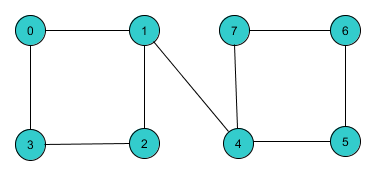
\includegraphics[scale=0.6]{graphics/LP0.png} 
	  \caption{Initial graph}
	  \label{lpa}
	\end{figure}
	  \begin{figure}[!hb]
	  \centering
	  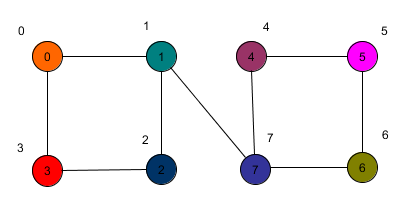
\includegraphics[scale=0.6]{graphics/LP1.png} 
	  \caption{First Iteration}
	  \label{lpa}
	\end{figure}
	\begin{figure}[h]
	  \centering
	  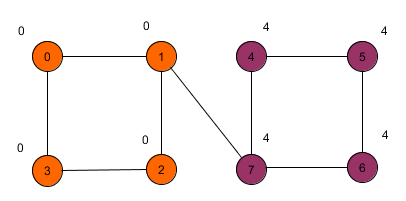
\includegraphics[scale=0.6]{graphics/LP2.png} 
	  \caption{Final Iteration}
	  \label{lpa}
	\end{figure}
	
  According to \cite{a:comm}, this algorithm presents some advantages such as it doesn't require parameter, it is easy to implement, fast to execute for large networks, and able to detect valid clusters even in random graphs. However, it may lead to assigning the same label to disconnected communities.

\subsubsection{Kmeans} \label{kmeans}
Kmeans is an unsupervised learning algorithm that aims to organise data from a given training set into few clusters.\ The Kmeans algorithm proceeds in two steps: First $K$ data items from the set of data points are randomly chosen as initial centroids, then, in the second step, each data point is assigned to the cluster which has the closest centroid and each cluster centroid is moved to the mean of the points assigned to it.\ This second step is repeated until all data points are assigned to one of the $K$ clusters.\\

			The Kmeans algorithm proceeds in two steps: \\
			- First K data items from the set of data points are randomly chosen as initial centroids. \\
			- In the second step, each data point is assigned to the cluster which has the closest centroid according to a chosen distance measure and each cluster centroid is moved to the mean of the points assigned to it. This second step is repeated until all data points are assigned to one of the K clusters. \\ Figure \ref{expl1} illustrates those steps. The circles refer to the datapoints and the triangles to the centroids. The datapoints with the same color belong to the same cluster.
				\begin{figure}[h!]
					\centering
					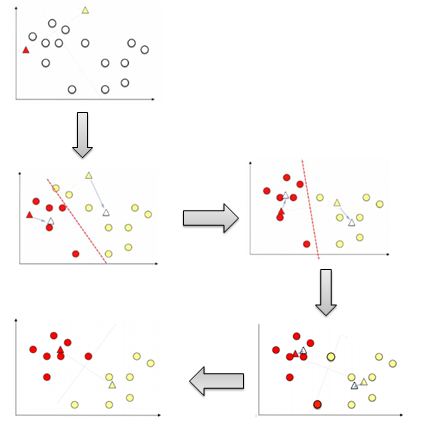
\includegraphics[scale=0.7]{graphics/expKmeans.PNG} 
					\caption{KMeans clustering example\cite{a:kmeansExple}} \label{expl1} 
				\end{figure}

			\textbf{- Silhouette Value:}
			
				A silhouette is a graphical display for partition techniques which shows  which objects lie  well within their cluster, and which not. The average silhouette width provides an evaluation  of clustering validity and might be used to select an 'appropriate' number of clusters \cite{a:silhouette}.\\
			 For each data point $i$, the silhouette $s(i)$ is given by the equation \ref{SilEq}:
				
				\begin{equation} 
					s(i)=\frac{b(i)-a(i)}{\max(a(i),b(i))} 
					\label{SilEq}
				\end{equation}
						
				where $a(i)$ is the average dissimilarity of $i$ with all other data within the same cluster and $b(i)$ is the lowest average dissimilarity of $i$ to any other cluster, of which $i$ is not a member.
						
						
						The instances are colored according to which cluster they belong to.
						the centroid values are recomputed according to the euclidean distance
\subsection{Supervised Learning}
In supervised learning, the training data you feed to the algorithm includes the desired
solutions, called labels.\\
A typical supervised learning task is classification.
Figure \ref{class} illustrates an example of a classification task: the system is trained with many labeled images, the label can be "airplane" or "car", the machine-learning process analyzes those labeled images and builds a model. This model is then used by the prediction process to classify unlabeled images. All the images were correctly labeled.
				\begin{figure}[h!]
					\centering
					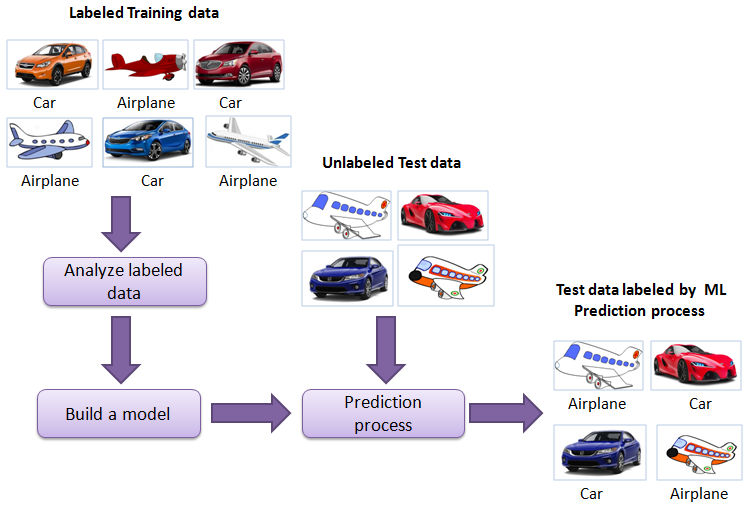
\includegraphics[scale=0.7]{graphics/classification.PNG} 
					\caption{Workflow of a classification example} \label{ref} 
				\end{figure}


	\subsubsection{Logistic Regression}	
	
	\subsubsection{Support Vector Machines}
		\label{svmSection}

			Support Vector Machines have been introduced in 1992 at the COLT conference by Boser, Guyon, Vapnik as a supervised learning approach used to solve classification and regression problems \cite{a:colt92}.

			The simplest kind of support vector machines called Linear SVM aims to find a hyperplane that optimally separates the training vectors into two classes by achieving the maximum separation, such that it will be equidistant to both datasets.\ Support vectors are defined to be a subset of the training data having the minimum distance to the hyperplane.\ An example of a simple linear SVM is illustrated in Figure~\ref{svm}.
				
				\begin{figure}[h!]
					\centering
					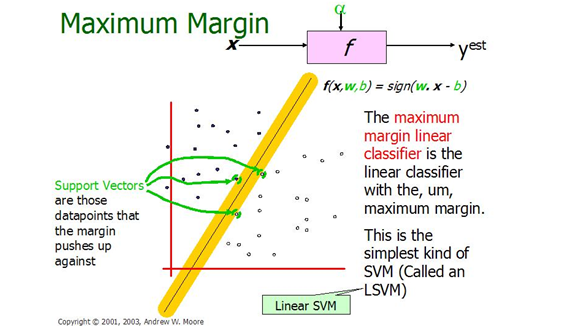
\includegraphics[scale=0.7]{graphics/LSVM.PNG} 
					\caption{Linear Support Vector Machines \cite{a:SvmSlides}} \label{svm} 
				\end{figure}

			The goals of SVM are separating the data with a hyper plane and extend this to non-linear boundaries when the data is far from linear and the datasets are inseparable by using the kernel methods that allow SVMs to form nonlinear boundaries, by non-linearly mapping the input data to a high-dimensional space.\ The new mapping is then linearly separable \cite{a:Nello:Svm} \cite{a:Tom:MachineLearning}.

			The kernel functions enable operations to be performed in the input space rather than the potentially high dimensional feature space.\ Various kernel functions can be used \cite{a:Nello:Svm}, such as: \textit{Polynomial}, \textit{Gaussian Radial Basis Function}, as well as \textit{Exponential Radial Basis Function}.
\chapter{State of the Art}
%related work. Present state of research and applied solutions concerning the different %aspects relevant to the thesis. Approximately 10 to 15 pages.\\
%During the last decades, several researchers were interested in the topic %identification field of written texts, because recognizing text topics is a primary %step of other text mining fields.

This chapter gives an overview of existing conducted research that deal with the problem of concept detection from a given dataset.\\ The developed approaches of solving this problem depend on the dataset type. This chapter is divided into two sections. The first section deals with existing approaches on text datasets whereas the second section deals with existing approaches on image and video datatsets.
\section{Concept Detection in Text Datasets}
A lot of approaches were developed to detect concepts from texts. For instance, we can distinguish between Term Frequency-Inverse Document Frequency (TF-IDF) based approaches, ontology based approaches and graph based approaches.
\subsection{TFIDF based approaches}
\subsubsection*{TF-IDF }
TF-IDF stands for term frequency-inverse document frequency and it was first presented in 1973 in \cite{a:tfidf}. TF-IDF is the most common term weighting scheme that evaluates the word importance to a document in a collection.\\
We suppose we have a query term t and a document d. The term frequency $tf_{t}(d)$ depends on the number of occurrences the term t appears in the document d and is calculated as follows: 
	\begin{equation}
	tf_{t}(d)= \frac {Number\ of\ occurences\ of\ the\ term\ t \ in\ the\ document\ d}{Total\ number\ of\ terms\ in\ the\ document}
	\end{equation}
With the raw term frequency, all terms are considered equally important when it comes to assessing relevancy on a
query. To attenuate the effect of too often occurring terms in the collection, the term frequency weight of a term t is reduced by the document frequency of the term t $df_{t}$, defined to be the number of documents in the collection that contain a term t.
Therefore, the inverse document frequency is defined as follows:
	\begin{equation}
		idf_{t} =  \log \frac {N}{df_{t}}
	\end{equation}
where N is the total number of documents in a collection. Thus the idf of a rare term is high, whereas the idf of a frequent term is likely to be low.
By combining those twos definitions we get the following composite weight:
	\begin{equation}
		tf{\small -}idf_{t}(d)= tf_{t,d}\cdot idf_{t}
	\end{equation}
%This metric was further enhanced, for instance in \cite{a:novel} a TF-IDF based weighting scheme to effectively rank the relevance of query terms to a document was developed. Their weighting scheme combines two term frequency components, one that tends to prefer long documents and another one that tends to prefer short documents based on the length of the corresponding query.\\  The scoring formula  that calculates the similitude between the query Q and the document D is depicted in \ref{eq1}:\\
%\begin{equation}
%  Sim(Q,D)=\sum_{1}^{|Q|} TFF_{q_{i},D}*TDF_{q_{i},C}
%\label{eq1}
%\end{equation}
%TFF stands for Term Frequency Factor and is obtained by combining the two factors as shown below:
%\begin{equation}
%	TFF(q_{i}, D)=w*BRITF(t, D)+(1-w)*BLRTF(q_{i}, D)
%\end{equation}
%where  $0<w<1$ and is set to: $w = \frac{2} {1+ \ln(1+|Q|)}$.\\
%\begin{equation}
%BRITF(q_{i},D)= \frac{RITF(q_{i},D)} {1+RITF(q_{i},D)}
%\end{equation}
%$BRITF(q_{i},D)$ has tendency to prefer long documents and RITF is the Relative Intra-document TF and it is defined as follows:
%\begin{equation}
%RITF(q_{i},D)=\frac{log2(1 +TF(q_{i}, D))}{\ln(1 +Avg.TF(D))}
%\end{equation}
%where TF($q_{i}$, D) denotes the frequency of the term $q_{i}$ in D and Avg.TF($q_{i}$,D) denotes the average term frequency of D.
%\begin{equation}
%BLRTF(q_{i}, D)=\frac{LRTF(q_{i}, D)}{1+LRTF(q_{i}, D)}
%\end{equation}
%LRTF is the Length Regularized TF.  $BLRTF(q_{i}, D)$ prefers short documents and longer queries are encountered.
%\begin{equation}
%LRTF(q_{i}, D)=TF(q_{i},D)×log2(1+ \frac{ADL(C)}{len(D)})
%\end{equation}
%where ADL(C) is the average document length of the collection and len(D) is the length of the document D.\\ 
%The average elite set term frequency AEC is defined as follows:
%\begin{equation}
%AEF(q_{i},C)=\frac{CTF(q_{i},C)}{DF(q_{i},C)}
%\end{equationj
%where CTF(t,C) denotes the total occurrence of the term t in the entire collection.\\
%The final term discrimination value of termt is computed as:
%\begin{equation}
%TDF(q_{i},C)=IDF(q_{i},C)×\frac{AEF(q_{i},C)}{1+AEF(q_{i},C)}
%\end{equation}
%C denotes the collection, CTF(t,C) denotes the total occurrence of the term t in the entire collection. \\
\subsubsection*{Concept Keyword Term Frequency/Inverse Document Frequency}
A TF-IDF based metric called Concept Keyword Term Frequency/Inverse Document Frequency ( ckTF/IDF ) was presented in \cite{a:ck} to efficiency mine concept keywords from identifiers present in the software source code. They used this metric to extract the concept keywords from udos \cite{a:udos}, an educational operating system consisting of 5,000 lines in C code.\\
\textbf{- Concept Keyword:}\\
concept keywords are a small subset of the words in identifiers and that represent a key concept that can aid in program understanding.\\
The authors distinguished between three kinds of concept keywords:
\begin{itemize}
\item [-] Ideal concept keywords: they prove to enhance program understanding by performing an objective measurement. 
\item [-] Human-selected concept keywords: are words that the code user believes they improve program understanding. For instance, \emph{dirent}, which implies “directory entry” is a human selected concept keyword.
\item [-] Machine-extracted concept keywords: is an algorithm that aims to extract keywords that are approximate to the human selected ones.
\end{itemize}
\textbf{- Definition of the ckTF/IDF method:}\\
The ckTF/IDF method treats one source file as a document. It quantizes tf(t,d) and idf(t) into 0 or 1. The idf(t) is defined as follows:\\
\begin{equation}
IDF(t) = \left\{ \begin{array}{rcl}
1 & \mbox{if} &
1 \leq df(t) \leq n  \urcorner isprefix(t)\\ 0 && otherwise
\end{array}\right.
\end{equation}
where df(t) is the document frequency of term t, n($\geq 1$) the threshold (default is 1) to quantize tf(t, d) and idf(t) and isprefix(t) predicate is true if and only if t is a prefix for all its occurrences. The metric assumes that prefixes are unlikely to be concept words, for example in the identifier "read\_dirent" from udos \cite{a:udos}, read is a prefix and is a generic verb not a concept keyword, whereas dirent is concept keyword.  \\The term frequency TF(t) in all documents.
\begin{equation}
tf(t) = \left\{ \begin{array}{rcl}
1 & \mbox{if} & \in d, tf(t, d) > n \\ 0 && otherwise
\end{array}\right.
\end{equation}
The word weight for ckTF/IDF is: 
\begin{equation}
w(t) = tf(t)* idf(t)
\end{equation}
A term t is selected as a machine-extracted concept keyword if w(t) = 1.\\
If we suppose that n=1 (the default value) then \textit{w(t)}=1 if t exists in only one document, it is not a prefix and there is one document where t occurs more than once. \\
The authors proposed a method to compute \textit{w(t)} in a fast way. They defined two flags for each term: a local frequency denoted \textit{local(t)} and a global frequency flag denoted \textit{global(t)}. 
After dividing all identifiers in source code into terms by using some delimiters like underscores, the two flags are computed for each term as follows: 
\begin{itemize}
\item [-] if a term t is found twice in a document then local(t) is set. 
\item [-] if this term t is found in two documents then global(t) is set. 
\item [-] \textit{w(t)}= 1 if local(t) is set, global(t) is clear, and the term is not a prefix otherwise \textit{w(t)}= 0. 
\end{itemize}
\textbf{- Performance evaluation:}\\
The authors developed a framework called Identifer Exploratory Framework (IEF) for the ckTF/IDF method.
To evaluate the performance of the ckTF/IDF method, the authors applied the ckTF/IDF and TF/IDF methods to their educational operating system udos’s source code, around 5,000 lines in C \cite{a:udos} and compared the concept keywords extracted by a human programmer with that found by the algorithm.  Therefore, they computed the performance metrics Accuracy and Coverage, which they defined as follows: 
\[Accuracy = \frac{C_{r}}{C_{m}}\]
where $C_{r}$ is the total number of concept keywords that both human and algorithm have chosen and $C_{m}$ is the total number of all machine extracted concept keywords.
\[Coverage = \frac{C_{r}}{C_{h}} \]
where  $C_{h}$ is the total number of human extracted concept keywords. \\
For the ckTF/IDF method, they achieved an accuracy of 57\%  and a coverage of 26\%, whereas for the TF/IDF method, they obtained as accuracy of 28\%  and a coverage of 13\%. Thus, ckTF/IDF delivers twice better accuracy and coverage than TF/IDF. \\
The authors have also applied the ckTF/IDF and TF/IDF methods on the Ruby interpreter to compare the execution speeds and found that ckTF/IDF is about 6 times faster than TF/IDF.
 
\subsection{Ontology based approaches} 
In this section, we will present two ontology based approaches to detect documents' concepts. First, let us define what is an ontology.
\subsubsection{What is an ontology?}
According to R. Studer et al., an ontology as a formal, explicit specification of a shared conceptualization \cite{a:def}. In other words, an ontology is composed of a set of vocabularies used to explicitly and
consensually describe a topic area and a set of explicit hypotheses on the meaning of
terms. It is expressed as a set of objects and the relationships between them and is
described in a formal language.\\ 
\subsubsection{Ontology based method for topic identification of learning materials}
The authors in \cite{a:ont} presented an ontological approach to automatically identify major topics covered in learning materials, also the subject and discipline to which those topics belong and relevance of the topic in the learning material as compared to other topics present in the same document are also discovered.
\begin{description}
\item[- Proposed approach:]
	
		The system stores the domain ontologies of various subjects, depicting the topics and terms relating to the subject and the relationships between them. For instance, Figure \ref{ont} shows an example of an ontology of the computer science subject.
				\begin{figure}[h!]
					\centering
					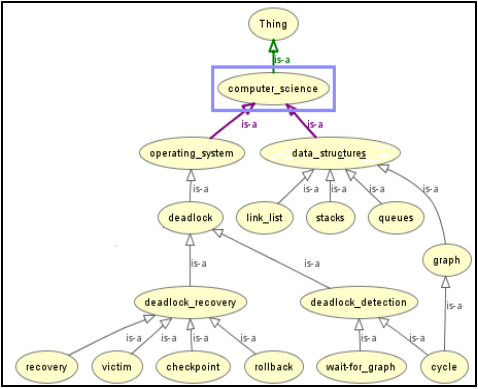
\includegraphics[scale=0.7]{graphics/ontology.PNG} 
					\caption{Domain Ontology of the subject Computer Science \cite{a:ont}} \label{ont} 
				\end{figure}
The authors designed the domain ontology with multiple layers defined as follows:
				\begin{itemize}
					\item[-] The top layer contains disciplines like Computer Science.  
					\item[-] The second layer contains Subjects under that discipline. 
					\item[-] The third layer contains the broad topics covered under that subject. \\
				\end{itemize}
					Topics again can contain sub-topics. These subtopics may be again represented by collection of various terms.
Figure \ref{workfow} depicts the workflow for the topic extraction process. 
                \begin{figure}[h!]
					\centering
					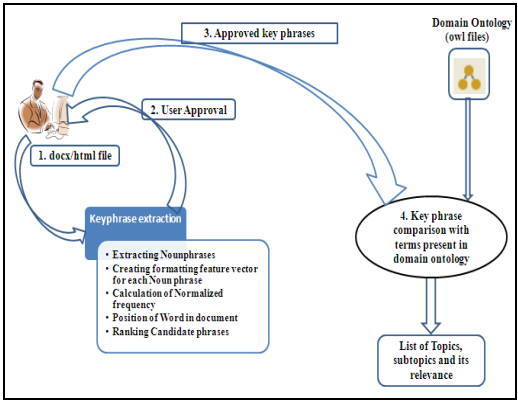
\includegraphics[scale=0.7]{graphics/workflow.PNG} 
					\caption{Workflow of the topic extraction process \cite{a:ont}} \label{workfow} 
				\end{figure}
After the user submits doc or html files, the Standford Parser \cite {standford} skimd these document for noun phrases, the stop words are deleted from those phrases which generates keyphrases that are ranked according to word frequency and displayed for user approval. These approved keyphrases are compared to the terms present in the domain ontology. If the domain ontology contains these keyphrases, then the OWL Parser retrieves the corresponding topics and subtopics are listed out and the relevance of document with respect to topic(s) /subtopic(s) 
enclosed in the learning material is calculated as follows:  \\	
 \[Relevance_{topic}(document)= \frac{number\ of\ its\ key\ terms\ identified\ under\ the\ topic/subtopic}{Total\ number\ of\ key\ terms\ identified\ in\ the\ entire\ document} \] 
Document can be characterized using the topic with higher relevance. 
\item[- Performance evaluation:]
		
		Documents consisting of 200 learning materials of different subjects were processed by the developed tool. The performance evaluation was done in two phases:
\begin{itemize}
\item [-] First phase: \\
The tool generated topics/subtopics were compared to those listed by subject experts. The authors used the F-score metric to evaluate the results. It is defined as follows:
\[F_{\beta} = \frac{(\beta^{2}+1) \cdot Precision \cdot Recall}{\beta^{2} \cdot Precision + Recall}\]
$\beta$ = 1 given precision and recall equal weights. \\
Precision and Recall are defined as follows:
\[Precision = \frac{Number\ of\ topic(s)/subtopic(s)\ identified\ correctly\ by\ the\ system } { Total\ topic(s)/subtopic(s)\ generated\ by\ the\ system}\] 
\[Recall = \frac{Number\ of\ topic(s)/subtopic(s)\ identified\ correctly\ by\ the\ system} {Number\ of\ topic(s)/subtopic(s)\ identified\ by\ the\ authors}\]
\item [-] Second phase: \\
In this phase, the topics/subtopics that were generated by the system but not listed out by the authors are shown to the authors for approval.
\end{itemize}
\end{description} 
Strict and lenient evaluations were performed. In strict evaluation, while comparing the system generated output with the expert list of topics/subtopics, the partially matched topics/subtopics are considered not found, whereas in lenient evaluation, they considered as matched. The obtained results are:
\begin{description}
\item[- Strict evaluation:]  

\begin{itemize}
\item [{\large $\cdot$}] Precision: 0.5057541
\item [{\large $\cdot$}] Recall: 0.8015656
\item [{\large $\cdot$}] Fscore: 0.63
\end{itemize}
\item[- Lenient evaluation:] 

\begin{itemize}
\item [{\large $\cdot$}] Precision: 0.6273393
\item [{\large $\cdot$}] Recall: 0.9609625
\item [{\large $\cdot$}] Fscore: 0.76
\end{itemize}
The authors have agreed on 82.3\% of the generated system topics/subtopics.
\end{description}

\subsubsection{A Wikipedia ontology based approach for automatic topic identification}
The authors in \cite{a:ont2} extracted the background knowledge from Wikipedia, and convert it into a structured Wikipedia Hierarchical Ontology (WHO) and presented an approach to automatically identify the documents' topics using this ontology.\\
Wikipedia categories were used to represent the WHO concepts, then the representative articles were gathered and organized for each concept so that they can be used to identify the relevant terms for that concept. After that the articles were cleaned by removing all kinds of formatting, the stop words were removed and the words were stemmed. After the preprocessing of the articles, a weight is assigned for each term
based on its importance to the concept according to the following equation:
\begin{equation}
TF-ICF = TF * \log(ICF)
\end{equation}
where TF stands for the Term Frequency, it is the number of occurrences of a term in a concept divided by the total number of terms in that concept, and ICF is the total number of concepts divided by the number of concepts that contains this term.  After the document-term matrix D is generated, the concept-term matrix C of the specific subset of concepts that we are interested in is extracted from WHO and matrix $C^{*}$ is formed.\\
The document-concept similarity matrix S is calculated as follows:\\
\begin{equation}
S = DC^{*T}
\end{equation}
\subsection{Machine learning based approaches}
In this section, we will give an overview of the Label Propagation Algorithm, that was used as a clustering algorithm in our approach and then present an example of a machine learning based approach.
	
     \subsubsection{Kmeans based Algorithm}
	The authors in \cite{a:kmeans} applied the Kmeans clustering algorithm to deal with the problem of topic detection. In their approach, they used the Vector Space Model for topic representation, K-means algorithm for text clustering and the Topic Detection and Tracking (TDT) method for performance evaluation. Figure \ref{proto} depicts the architecture of the topic detection prototype.
	\begin{figure}[h]
	  \centering
	  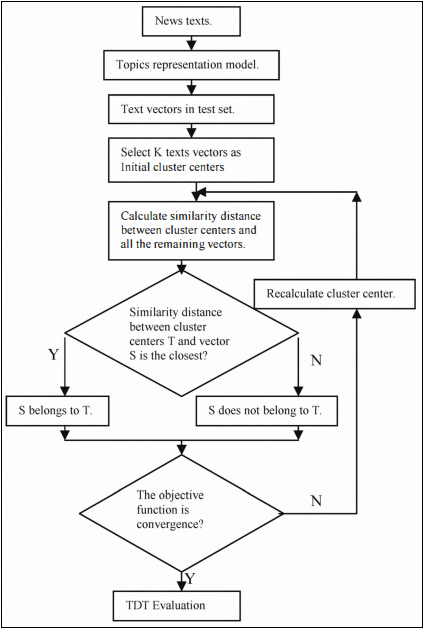
\includegraphics[scale=0.7]{graphics/proto.png} 
	  \caption{Architecture for Topic Detection Prototype System}
	  \label{proto}
	\end{figure}
In the remainder of this section, we will explain this diagram  by going through each component.
 \begin{enumerate}
	\item \textbf{Topics Representation Model:\\}
	 The topic model is a statistical language model that reveals a hidden thematic structure of the text collection and finds a highly compressed representation of each document by a set of its topics. It is based on the idea that documents are mixtures of topics, where a topic is a probability distribution over words \cite{a:Huang2008} \cite{a:b} \cite{a:Daud2010}.\\ 
	Several topic modeling techniques were introduced in the literature such as Latent Semantic Analysis (LSA), Latent Dirichlet Allocation (LDA) and the Vector Space Model (VSM), which was applied in this prototype.\\
	The Vector Space Model was introduced in 1971 by Gerard Salton \cite{a:vsm}. In this model each document in a collection is represented as a vector in a vector space, the distance between the vectors is calculated and the vectors that are close to each other are semantically similar. 
	To express a document text as a vector, the words are first extracted and the stop words are eliminated then the TF-IDF metric is calculated for each word in the document. \\
	If we suppose the training set contains n terms after removing the words, then each document d in the training set is expressed as an n-dimensional feature vector V(d).
	\begin{equation}
	V(d)=\left(t_{1},w_{1}(d);t_{2},w_{2}(d);\cdots t_{n},w_{n}(d)\right)
	\end{equation}
	Where $t_{i}$(i=1,2,⋯,n) is term i, and $w_{i}$(d)(i=1,2,⋯,n) is the weight of the text d, calculated using the cosine normalized version of the TF-IDF algorithm.
	\begin{equation}
		{\cal W}_{i}(d)={-tf_{i}(d)\times\log({q}/q_{i})\over \sqrt{\sum\limits_{i}(tf_{i}(d)\times\log(q/q_{i}))^{2}}}
	\end{equation}
 
A feature selection algorithm called Information gain was then applied to select an informative subset of text terms.\\ Information gain (IG) measures the amount of information in bits about the class prediction by knowing the presence or the absence of a term in a document \cite{a:yangcomp}.\\
  For the term t and topic c, information gain \cite{a:yangcomp} is defined as follows: \\
 \begin{equation}
IG(t)=-{\sum}_{i=1}^{m}P(c_{i})\log P(c_{i})+P(t){\sum}_{i=1}^{m}P(c_{i}\vert t)\log P(t)+P(\bar{t}){\sum}_{i=1}^{m}P(c_{i}\vert \bar{t})\log P(c_{i}\vert \bar{t})
\end{equation}
Where $P(c_{i})$ is the probability that the topic i appears in the corpus, P(t) is the probability that a topic includes the term t, $P(c_{i}\vert t)$ is the conditional probability that the term t belongs to the topic i when the topic includes term t, $P(\bar{t})$ is the probability that a topic does not include the term t, $P(c_{i}\vert \bar{t})$ is the conditional probability that the term t belongs to the topic i when the topic does not include term t, and parameter m is the number of topics.
		\item \textbf{KMeans Algorithm for Text Clustering:\\}
		An overview of the Kmeans algorithm was given in \ref{kmeans}. In the case of text clustering the Kmeans algorithm proceeds as follows: 
\begin{itemize}	
\item [-] First $K$ data items from the set of data points are randomly chosen as initial centroids or mean of a topic. 
\item [-] In the second step, each remaining data point is assigned to the cluster which has the closest centroid according to the cosine distance between the text vectors, which is defined as follows:
		\begin{equation}
			Dis(d_{i},d_{j})=1-Sim(d_{i},d_{j})
		\end{equation}
			
	Where $d_i$ is text feature vector i, $d_j$ is text feature vector j and Sim($d_{i}$,$d_{j}$) is the cosine similar function between the document i and document j and is defined according to VSM as follows:
		\begin{equation}
 			Sim(d_{i},d_{j})={\sum\limits_{k=1}^{n}{\cal W}_{ik}\times {\cal W}_{jk}\over\sqrt{\sum\limits_{k=1}^{n}{\cal W}_{ik}^{2}}\times\sqrt{\sum\limits_{k=1}^{n}{\cal W}_{jk}^{2}}}
		\end{equation}
where n is the dimension of feature vectors and ${\cal W}_{ik}$ is the weight of the feature k in document i calculated according to the TF-IDF algorithm.  The smaller the cosine distance between the two texts is, the more similar they are.	
\item [-] Then, each cluster centroid is moved to the mean of the points assigned to it.
This step is repeated until all data points are assigned to one of the $K$ clusters.
\end{itemize}
		\item \textbf{TDT Evaluation:\\}
		If a topic could not be detected by the system, the resulting error is called "missed detection error", but if a system detects a wrong topic, the error is called "false alarm"\cite{a:tdtmetric}. The official evaluation measure of TDT is based on a cost function, which is a weighted combination of miss and false alarm rates \cite{a:tdtmetric}:
	\begin{equation}
C_{Det} = C_{Miss}\cdot P_{Miss}\cdot P_{target} + C_{FA}\cdot P_{FA}\cdot P_{non-target} 
	\end{equation}
$P_{target}$ is the prior probability that the topic is correctly detected ($P_{non-target}$ = 1 - $P_{target}$). $C_{Miss}$ and $C_{FA}$ are user defined  values that reflect the cost associated with miss and false alarm errors respectively and $P_{Miss}$ and $P_{FA}$ are the probabilities of a Miss and a False Alarm.
The cost parameters used in the evaluation are:  $P_{target}$= 0.02, $C_{Miss}$ = 1.0, $C_{FA}$=0.1.
The $C_{Det}$ value is normalized as follows:
	\begin{equation}
			(C_{Det})_{Norm} = C_{Det}/\min(C_{Miss}\cdot P_{target}, C_{FA}\cdot P_{non-target})
	\end{equation}	
The authors defined the $S{\_}Tracking{\_}P$ metric to test topic tracking overall performance. This metric is calculated as follows:
			\begin{equation}
	S{\_}Tracking{\_}P={\sum\limits_{i=1}^{m}((C_{Det})_{Norm})_{i} \over m}
			\end{equation}
	where m is the number of topics, and $((C_{Det})_{Norm})_{i}$ is TDT evaluation scores in topic i.
	\end{enumerate}  	  
	  
	  
\subsection{Graph based approaches}
A graph approach for topic identification called LIGA and two extensions that enhance its performance were introduced in \cite{a:arabic}. The tests were done on arabic datasets. 
The authors of \cite{a:arabic} applied the LIGA approach, which was first introduced in \cite{liga} for language identification, to identify the topics from the documents.

Figure \ref{liga} shows the different steps of the LIGA approach.

				\begin{figure}[h!]
					\centering
					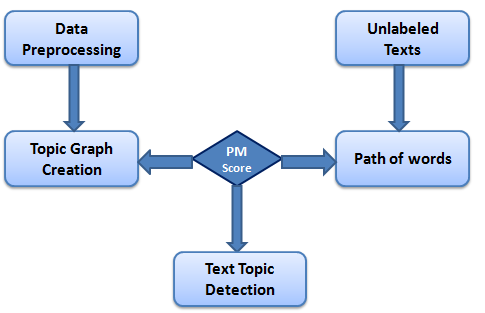
\includegraphics[scale=0.7]{graphics/LIGA.PNG} 
					\caption{LIGA Approach workflow} \label{liga} 
				\end{figure} 
				First the training documents are preprocessed by eliminating the foreign words and the stop words and stemming the rest of words. Then the LIGA approach is applied. This approach can be divided into two steps: model construction and document classification.
				\begin{itemize}
				\item [-] Model Construction:\\
				For each training document a graph, which corresponds to one topic called "topic graph" will be constructed. In this graph, each node contains a word and its number of occurrences in the training document, and each edge represents the link between two consecutive words in the training documents, and the weight of the edge represents the number of occurrences of these consecutive words. \\
				Let's take the example of the following sentence: " \textit{A sad movie is a movie that makes the viewer feel sad and cry} ". \\
				The corresponding topic graph is shown in Figure \ref{topic}.
				\begin{figure}[h!]
					\centering
					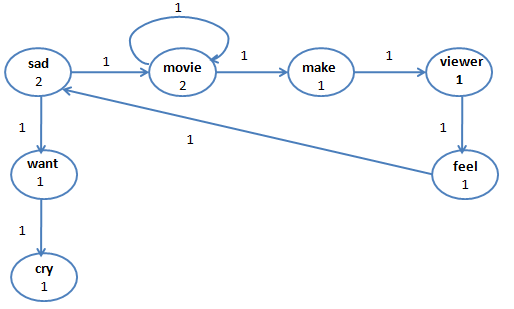
\includegraphics[scale=0.7]{graphics/topicGr.PNG} 
					\caption{Topic graph example} \label{topic} 
				\end{figure} 
				After prepocessing the sentence, the topic graph would be: 
				\item [-] Document Classification:\\
				The unlabeled texts are presented as a path of words, and the entire paths are matched onto the graphs and the similarity between them is computed using the Path Matching (PM) score. The PM score assigns an integer to each topic. All PM scores of all topics are initially initialized to 0.\\
				To compute the PM score, the path is traversed node by node. If a path node exists in a topic graph $G_{i}$ , then its weight is added to the PM score and if a path edge exists in the topic graph $G_{i}$ then its weight is also added to the PM score. The text topic corresponds to the topic graph having the highest PM score. \\	
				Let's take the example of the following sentence: " \textit{Titanic is one of the best sad movies ever made}." This sentence corresponds to the path of words presented in \ref{path}: \\
				\begin{figure}[h!]
					\centering
					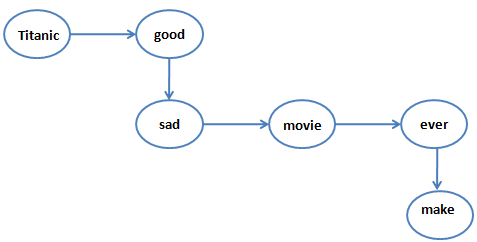
\includegraphics[scale=0.7]{graphics/path.PNG} 
					\caption{Word Path example} \label{path}
				\end{figure} 
					The words "sad", "movie" and "make" existed in the topic graph shown in \ref{topic} also the edge (sad,movie) existed in this topic graph. Thus $PM = weight(sad) + weight(movie)+ weight(make)+ weight((sad,movie)) = 5 $  			
				\end{itemize}
				
 
Another graph-based approache was introduced in \cite{a:wiki} which applies the Page-Rank algorithm on Wikipedia derived graph to decide the importance of a vertex within a graph. 
\section{Concept Detection in Image Datasets}
	A search engine that allows users to pose natural language queries, interpretes them and retrieves the corresponding images called GOOSE was presented in \cite{a:inter}. The user query is semantically interpreted, concepts are detected from the images and learned by matching these detected concept against the user query which he can refine. The user can also re-rank the results. Figure \ref{sys1} gives an overview of the system components which will be further explained.
\begin{itemize}
	\item Semantic Query Interpretation: \\
		The user query is first lexically analysed using the Stanford Typed Dependency parser \cite{a:parser} which transforms it into a direct graph where nodes are the words and the labeled edges depict the grammatical relations between the words. Let's for example take the sentence: "\textit{Find a brown animal in front of a red Mercedes}", the resulting  directed graph from depicted in Figure \ref{lexical}, where the grammatical relations: dobj, amod, det stand respectively for direct object, adjectival modifier and determiner.

\begin{figure}[!hb]
	  \centering
	  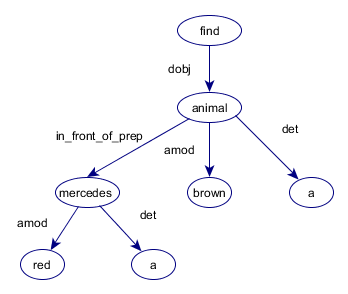
\includegraphics[scale=0.6]{graphics/standfordG.png} 
	  \caption{Lexical graph}
	  \label{lexical}
\end{figure}

	  	This lexical graph is then semantically interpreted by applying a set of rules to transform the lexical graph elements into objects, attributes,  actions, scenes and relations, according to the semantic meta-model depicted in \ref{model} which the authors defined.
This semantic Meta-model distinguishes objects that might bear attributes, take part in actions, occur in a scene and have relations with other objects.
\begin{figure}[!hb]
	  \centering
	  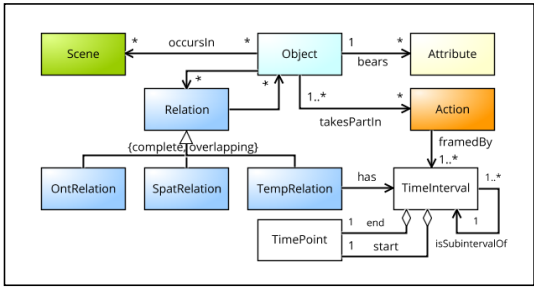
\includegraphics[scale=0.6]{graphics/SMM.png} 
	  \caption{Semantic Meta-model}
	  \label{model}
\end{figure}
After applying the semantic interpretation on the sentence: "\textit{Find a brown animal in front of a red Mercedes}", we obtain the graph shown in Figure \ref{sem}, where the cardinality 1 is derived from the determiner "the", which is in a singular form. The attribute "color" is derived from the adjectival modifier.  
	\begin{figure}[!hb]
	  \centering
	  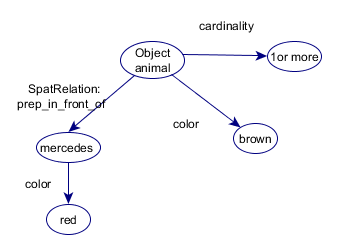
\includegraphics[scale=0.6]{graphics/attrG.png} 
	  \caption{Interpreted Graph}
	  \label{sem}
\end{figure}
	  This semantic graph is matched against the detected image concepts. If there is no exact match, the semantic graph is expanded using ConceptNet \cite{a:concept}, a large semantic graph representing common human knowledge and the way it is expressed in natural language. The words in ConceptNet are related through predicates such as: "IsA" and "Causes". These relations were selected to expand the semantic graph where the unknown concepts are matched against concepts from  ConceptNet, if a match is found, the matching concepts and their corresponding 'IsA' and 'Causes' relations are imported to the semantic graph. Otherwise, the expansion cycle goes through a second iteration. The expanded semantic graph of the user query is shown in Figure \ref{exp} where the green nodes are the concepts that were recognized before the expansion, the orange nodes are the concept nodes corresponding to expansions with ConceptNet and red nodes are the still unknown concepts after the expansion. An example of the colored semantic graph  for the query ‘Find a brown animal in front of a red mercedes’ is shown in Figure \ref{exp}. This graph corresponds to the structured query that the user can further refine.
	\begin{figure}[!hb]
	  	\centering
	  	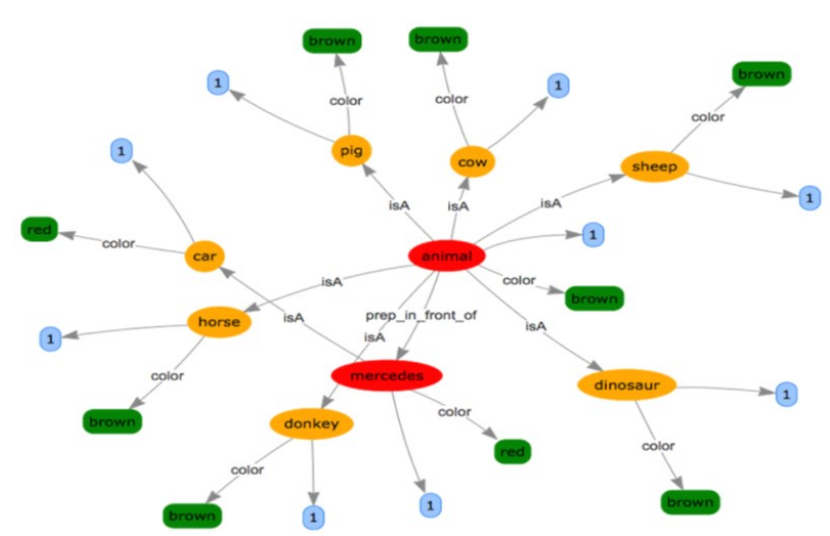
\includegraphics[scale=0.6]{graphics/expansion.png} 
	  	\caption{Expanded Semantic Graph of the query}
	  	\label{exp}
	\end{figure}
	  	
	 \item Concept Learning and Concept Detection: \\ 
	  	The system  automatically recognizes and localizes concepts in video using the R-CNN method, which stands for Region proposals with Convolutional Neural Networks, presented in \cite{a:rcnn}. \\ This method consists of generating region proposals, extracting a feature vector from each region and classify each region using SVM. In the following, we will go through each of those steps: \\
	 - Region Proposals generation: \\
	 around 2000 bottom-upt category-independent region proposals were extracted using the selective search method. 
\cite{a:J. Uijlings, K. van de Sande, T. Gevers, and A. Smeulders. Selective
search for object recognition.IJCV, 2013.}\\
	 - Features extraction:
	 a 4096-dimensional feature vector from each region proposal using a Convolutional Neural Network.
	 CNN  are ..\\
	 - Regions classification:
	 SVM ..
	  	
	  	 
	 
	
\end{itemize}
Finally the semantic graph is matched against the concepts that can be detected using the R-CNN algorithm. If a match exists, then the corresponding nodes in the graph are colored in green. Otherwise, the semantic graph is expanded using ConceptNet, a large knowledge base constructed by combining multiple web sources such  as DBpedia, Wiktionary and WordNet.\\
The authors of \cite{a:online} developed an algorithm for learning multiple consecutive tasks or Multi-Task Learning algorithm for video concept detection.\\ This algorithm exentded the Efficient Lifelong Learning (ELLA) Algorithm described in \cite{a:ella}. ELLA learns and maintains a shared basis for all task models. For each new task, the algorithm transfers knowledge through the shared basis to learn the new model, and refines the basis with knowledge from the new task to maximize the performance. The proposed algorithm was referred to as Efficient Lifelong Learning Algorithm with Label Constraint, it extends the ELLA algorithm by solving the objective function of ELLA using quadratic programming, adding a new label-based constraint that incorporates statistical information of pairwise correlations between concepts and instantiating ELLA with two base classifiers linear Support Vector Machines(SVM) and Logistic regression (LR). 
\chapter{Contribution}
After going through the background and the state of the art, in this section we will present our novel graph-based approach to detect the concept out of highly-linked large datasets.
In our model, the text datasets are first prepocessed then the training datasets are fed to our learning algorithm and finally the model is tested on new unlabled texts. In the remainder of this section, we will go through each of those steps.

\section{Preprocessing}
This step consists of preparing the datasets for further analysis. The words in the datasets are first extracted , stop words are removed, the rest of words are stemmed and lemmatised. Stemming is the process of replacing a word by its root independetly of the context of the word, for example, the words "connection", "connected" and "connectivity" will all be replaced by "connect" \cite{a:stem}. Lemmatisation consists also of determining the base form of a word called lemma depending on its context. For instance the lemma of "better" is "good" which won't be determined using the stemming technique \cite{a:lemma}.
Both stemming and lemmatisation are word normalization techniques that will help us determine the occurence of the word and all its derivatives in the dataset.
Let's take the following sentence: \\
	It is no secret that fans of Chinese food often find it addictive. S1\\
After eliminating the stop words, stemming and lemmatizing the sentence, we obtain the following list of words: \\
secret, fan, chines, food, find, addict



\section{Approach}
\subsection{Model construction and learning}
A training graph having as vertices the set of preprocessed words in the dataset and three kinds of edges: "follow", "child" and "implication" is construced.
For each sentence, the follow edges are built between consecutive words in each sentence. The child edges depict the grammatical relationships between the words. Each sentence is then presented to a person that enters the list of concepts he understands from it. An implication edge between each word of the sentence and each understood concept is added to the graph.
Once the training graph is constructed, the clustering algorithm "Label Propagation" is applied on it. Each obtained cluster is colored with a different color. \\
Let's assume a user understands the concepts:  "food, fans" from sentence S1:\\
After lemmatizing and stemming those words, we obtain the following list of implications: fan, food. \\
As a result, we obtain the following training graph:



\begin{figure}[!hb]
	  \centering
	  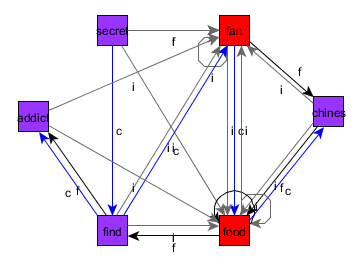
\includegraphics[scale=0.6]{graphics/sentence.png} 
	  \caption{Training graph}
	  \label{fig:trainingGraph}
\end{figure}
The implication vertices are colored in red.	  

\subsection{Model testing}
After preprocessing the testing texts, a graph containing the "follow" and "child" edges is constructed in the same way. Then this graph is matched to the training graph, if there are some common nodes in both graphs, then the "implication" edge between the node and its corresponding concept is copied from the training graph to the tesing graph.
\begin{figure}[!hb]
	  \centering
	  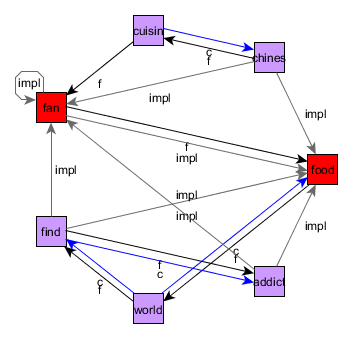
\includegraphics[scale=0.6]{graphics/onlytestsentence.png} 
	  \caption{Testing graph}
	  \label{fig:trainingGraph}
\end{figure}
The induced implication vertices are colored in red.





%\chapter{Self-Organizing Random Walk-Based CkDS Construction}

Most important chapter of the thesis. Describes what the author adds to state of the art. Discusses intuition, motivation, describes and reasons about necessity of proposed elements. Defines theses based on reasonable assumptions. Discusses relevant aspects of contribution. Approximately 30 to 40 pages. Can be split into multiple chapters.

This is an example text with figures, definitions and so on.

\label{bickds}

After a review of background information and state of the art in the previous chapters, this chapter introduces a novel approach for the construction of connected $k$-hop dominating sets (CkDS) in wireless sensor networks (WSNs). To cope with the resource restrictions of this network class, as reviewed in Section \ref{sechardware}, the biologically-inspired, self-organizing protocol employs methods and exhibits properties which are inherent in many biological systems. It is inspired by the general technique of random walks and, in particular, by the flight behavior of ovipositing Pieris rapae, which efficiently solves the coverage problem in nature by employing random walks. The proposed approach is the first protocol for the construction of connected dominating structures, including CDS and CkDS, to adopt random walks to wireless networks. In \cite{own092}, the central contribution of this chapter was published recently.



The first section of this chapter presents an overview of the inspiration and the design considerations for the introduced CkDS construction method. Thereafter, Sections \ref{bickds_sec_outline}--\ref{sb2} provide a detailed description of the proposed protocol, before Section \ref{ourprotdisc} discusses its behavior.



\section{Outline}\label{bickds_sec_outline}    \label{ourprot}\label{sec_o} \label{core}

The proposed protocol consists of two intertwined behavior blocks: in the first, a dominating set is constructed, in the second, this set is connected to become a CkDS. Each of the blocks is further subdivided into two subblocks: exploration and construction.  

Assuming a network without a dominating set, the first behavior block (Section \ref{sb1}) starts with the exploration subblock, in which exploration agents roam the network in order to find candidate segments for the addition to the dominating set. Their movement pattern is similar to the discussed movement pattern of P. rapae (Section \ref{secbpr}). If certain conditions are satisfied, a candidate segment is added to the dominating set by agents from the construction subblock. As a result of the parallel construction operations of this block, a dominating set is produced.



While the agents in the first behavior block still explore and construct, the operations specified by the second behavior block (Section \ref{sb2}) are already executed. Agents from the exploration subblock perform random walks similar to their relatives in the previous block and in nature, but with restrictions which increase the probability to find a candidate path for the connection of two disconnected segments of the already existing dominating set. A rule which forces these agents to start only from dominating nodes is, for example, part of these restrictions. In the construction subblock, agents construct connections between dominating set segments that appear disconnected, selecting from the candidate paths found by exploration agents. To improve the quality of the solution, for instance, there are mechanisms that help to avoid the creation of redundant interconnections. As a result of these behavior blocks, a CkDS is produced.

The description of the proposed protocol is organized as follows: All necessary definitions used later in the text are introduced in Section \ref{cds_ckds_def}. The local data structures and next-hop candidate ratings utilized by the protocol are specified in Sections \ref{slds} and \ref{slr}. Subsequently, in Sections \ref{sb1} and \ref{sb2}, the two behavior blocks representing the core of the protocol are described in detail.

\section{Definitions}\label{cds_ckds_def}\label{sec_d}

A connected WSN is modeled as graph, using the following definitions:

\begin{definition}\label{defgpure}

An \emph{undirected graph} $G = (V,E)$ consists of a set of vertices $V$ and $E$, a set of edges $(u,v)$, where $u,v \in V$ and $u\neq v$. $(u,v)$ and $(v,u)$ are considered the same edge. If $(u,v)\in E$, then also $(v,u)\in E$.

\end{definition}

\begin{definition}\label{defcon}

A set of vertices $S\subseteq V$ in an undirected graph $G = (V,E)$ (according to Definition \ref{defgpure}) is \emph{connected}, if, between each pair of vertices $\{u,v\}$, with $u,v \in S$, there exists a path consisting only of vertices from $S$.

\end{definition}

The proposed protocol, similar to the related approaches, assumes bidirectional links, which are modeled as undirected edges constituting set $E$ in $G=(V,E)$. This assumption reflects the fact that usually unicasts need to be acknowledged at MAC level, which is only possible given bidirectional links. However, real links may be unidirectional, as implied, for example, by Figure \ref{bg_realtx} in Section \ref{seccom}. To cope with this, in the real-world, the network graph is simply stripped of unidirectional links (i.e.\ such links are ignored).


\begin{definition}\label{defg}

An \emph{undirected, connected graph} $G = (V,E)$ is an undirected graph according to Definition \ref{defgpure} whose set of vertices $V$ is connected under Definition \ref{defcon}.

\end{definition}

The following definitions assume an undirected, connected graph $G=(V,E)$ according to the above definition:

\begin{definition}\label{defpath}

A \emph{path} of length $l$ between $v$ and $u$ is a sequence of vertices $\langle v_0,v_1,v_2,\ldots,v_l \rangle$, such that $v=v_0$, $u=v_l$, $(v_{i-1},v_i) \in E$, and $i=1,2,\ldots,l$, with $v_0,v_1,v_2,\ldots,v_l \in V$.

\end{definition}

\begin{definition}\label{defadjacent}

Two vertices $v, u\in V$ are \emph{adjacent}, if there exists an edge $(u,v)\in E$.

\end{definition}

There are two \emph{vertex states}: \emph{dominating} and \emph{non-dominating}. 

\begin{definition}\label{defdomset}

A \emph{dominating set} $D \subseteq V$ is the set of all vertices $v\in V$ whose state is dominating.

\end{definition}

A connected $k$-hop dominating set (CkDS) is defined as in Definition \defref{defckds}.

 
\begin{definition}\label{defcenter}
 
 A vertex $v_c$ is also called a \emph{center}, if $v_c \in$ dominating set $D$, and there exist three edges $(v_c, v_1)$, $(v_c, v_2)$, and $(v_c, v_3)$, with $v_1, v_2, v_3 \in D$ and $v_c\neq v_1\neq v_2\neq v_3$. 
 
\end{definition}



Different neighborhood sets are defined as follows: 

\begin{definition}\label{defnall}

$N_w(v)$ contains \emph{all} vertices in the $w$-hop neighborhood of vertex $v$. 

\end{definition}

\begin{definition}\label{defndom}

$N_w^D(v)$ contains \emph{all dominating} vertices in the $w$-hop neighborhood of vertex $v$. 

\end{definition}

\begin{definition}\label{defnondom}

$N_w^n(v)$ contains \emph{all non-dominating} vertices in the $w$-hop neighborhood of vertex $v$. 

\end{definition}

\begin{definition}\label{defncenter}

$N_w^c(v)$ contains \emph{all} vertices called \emph{centers} in the $w$-hop neighborhood of vertex $v$. 

\end{definition}



\section{Local Data Structures}\label{slds}\label{sec_lds}

Each node $v$ maintains a field $d\in \{n,D\}$, which contains the state of the node: non-dominating ($n$) or dominating ($D$). Additionally, each node administers the following tables:

\begin{itemize}

\item \emph{Neighborhood Table $nTab(v_n)$:} This table includes the $1$-hop neighborhood of a node. The information in this table is used for the probabilistic next-hop selection by the initial exploration and connection exploration agents (IEAs and CEAs), as described in Sections \ref{sec_inhs} and \ref{sec_oonh}. An entry is associated with the neighbor $v_n$ (identified by its address) and contains the following fields: 

		\begin{itemize}

			\item $s$ records the state of $v_n$, i.e.\ whether it is dominating or non-dominating. This information can be obtained from a received broadcast sent by a state-changing node.
			
			\item $rssi$ records the received signal strength indication (RSSI)\abbrev{RSSI}{Received Signal Strength Indication} of $v_n$, assuming that it has been normalized adequately to reflect the approx.\ distance to $v_n$. The method for acquiring RSSI values is platform dependent.
			
			\end{itemize}

The addresses of $1$-hop neighbors can be, for example, obtained from an underlying WSN medium access control (MAC) protocol, such as \emph{S-MAC} \cite{ye02protocol} or \emph{SCP-MAC} \cite{ye06mac}, which is aware of the $1$-hop neighborhood, so that no additional overhead is incurred.  

\item \emph{Interconnection Table $iTab(v_s)$:} In order to enable the interconnection of 
dominating set segments in the second behavior block, when a connectivity exploration agent (CEA) $a_{CE}$ visits node $v$, $a_{CE}$ downloads its path and center information to $v$'s local interconnection table (see Section \ref{sec_pwfc}). When another CEA visits $v$, it can evaluate whether its interconnection table contains paths that lead to a dominating set segment which appears to be disconnected (see Section \ref{sec_oonh}). For each source node $v_s$, the entry has the following format:

\begin{itemize}
 \item $p$ records the path to dominating node $v_s$
 
 \item $cns$ contains the centers that are reachable via the dominating node $v_s$

\end{itemize}
 
Note that $p.length$ and $p.source$ return the length and the source (i.e.\ first) node of the path (this also applies to the path fields of agents). Further, if an entry has not been updated within $t_{itu}$ time, it is deleted.
		
\item \emph{Next-Hop Utilization Table $nhuTab(v_{s}, v_{n})$:} The utilization of next hops by connection exploration agents (CEAs) is recorded in the next-hop utilization table (see Section \ref{sec_pwfc}). After a CEA, originating from node $v_s$, selects its next-hop, it records its selection to this table. Thereafter, the probabilities assigned to next hops are influenced by this selection for other CEAs also originating from $v_s$ (see Section \ref{sec_nhsd}). \todoh{explain somewhere whhy association with vs} For a source node $v_s$ and a next-hop neighbor $v_n$, the entries contain only one field: 

\begin{itemize}

\item $uf$, the utilization frequency, which is initially $0$.

\end{itemize}

\item \emph{Center Distance Table $cdTab(v_c)$:} This table maintains information on center nodes within $CIPA_{mh}$-hops (along dominating nodes) of a node. It serves two purposes: first, it facilitates the rating of the connectivity of a dominating node (see Section \ref{sec_cr}), second, it enables CEAs to recognize dominating set segments that appear to be disconnected (see Section \ref{sec_nhsd2}). The entries of the center distance table, associated with a center $v_c$, contain only one field

\begin{itemize}

	\item $d$, recording the distance to $v_c$.
	
\end{itemize}

\end{itemize}


Note that not all tables are needed on all nodes. The center distance table is only maintained on dominating nodes, for instance. Moreover, most of the tables serve several purposes and may be utilized in combination: for example, a CEA evaluates the neighborhood, the next-hop utilization, and the interconnection tables to select its next hop (see Section \ref{sec_oonh}).


In order to refer to elements of these tables, this document employs several simple notations. Here are some examples for typical usage:

\begin{itemize}

		\item $v_a.nTab(v_b).rssi$ for the $rssi$ field associated with neighboring node $v_b$ in the neighborhood table of node $v_a$
		
		\item $v_a.iTab.v_s$: all source nodes in the interconnection table at node $v_a$
		
		\item $v_a.iTab.cns$: all $cns$ fields in the interconnection table at node $v_a$
		
\end{itemize}

\section{Next-Hop Candidate Ratings}\label{slr}\label{sec_nhcr}

In contrast to the existing CkDS approaches, reviewed in Section \ref{sotackds}, the proposed approach offers a seamless integration of next-hop candidate ratings, colluding with its probabilistic next-hop selection process. The ratings take into account the quality of a link (Section \ref{sec_lqr}) towards a potential next hop and its utilization properties (Section \ref{sec_ur}). Therefore, the proposed protocol achieves randomized connected coverage, while considering the quality and utilization of next-hop candidates. 

\done{what about energy rating above}

\subsection{Link Quality Rating} \label{sec_lqr}

The link quality rating has the following objectives: First, links that are expected to lead to successful transmissions more often should be preferred over links that are expected to yield lower transmission success rates. Second, from the links which are expected to lead to high transmission success rates, the ones should be preferred that cross as much distance as possible, so that fewer hops are needed to cover a certain area of the network.


In other words, the link rating aims at maximizing the additional amount of coverage of each link in a random walk, while, at the same time, it avoids links with low transmission success rates. Since a successful transmission implies a successful reception and vice versa, I will use the term \emph{reception success} to describe a successful transmission and reception of a frame or packet, as it is more common in the community.


Before introducing the proposed link rating, related, preparatory work by other authors needs to be reviewed briefly: As described in \cite{woo03} and \cite{zhao03performance}, two correlations can be observed: First, there is a positive correlation between received signal strength and reception success rate. Naturally, at the same time, a negative correlation between received signal strength and distance can be found. Note that for the sake of brevity, I will frequently use the abbreviation RSSI, short for \emph{received signal strength indication}, to refer to received signal strength.

The relationship between distance and reception success rate is depicted in Figure \ref{bickds_thresholds}, based on the data from \cite{woo03} for Berkeley Mica motes. In the figure, the rate of reception success is plotted as a function of distance. To obtain the data, the authors positioned a grid of nodes in an open tennis court at two feet (60.96 cm) distance in both dimensions. The nodes transmitted 200 packets at a rate of eight packets per second, with only one transmitter active at a given time and the remaining nodes receiving. It is evident from the figure ($a$ and $b$ are marked in the chart) that the distances can be divided into three categories:


\begin{description}
\item[0 to a] In this region, the probability that a frame/packet will be received successfully is very high. Thus this region should be preferred.

\item[a to b] Within these limits, there is an acceptable probability that a packet will be received successfully.

\item[b to $\infty$] In this area, the transmitted packet is likely not to be received. Therefore it should be avoided.

\end{description}

From the description above, it is evident that 

\begin{description}

\item[a] represents a distance threshold below which the reception success rates are excellent. Since there is a negative correlation between distance and signal strength, the RSSI value corresponding to this distance can be regarded as a threshold, labeled $r_{pr}$, above which the reception success can be expected to be excellent and therefore links with RSSI values greater $r_{pr}$ should be \emph{preferred}.

\item[b] identifies a distance threshold below which the reception success rates are acceptable. As there is a negative correlation between distance and signal strength, the RSSI value corresponding to this distance can be regarded as a threshold, labeled $r_{ac}$, above which the reception success can be expected to be acceptable and therefore links with RSSI values greater $r_{ac}$ should be \emph{accepted}.

\end{description}



The proposed link quality rating takes into account these considerations by categorizing links into three rating classes according to their RSSI values $r$ and the thresholds $r_{ac}$ and $r_{pr}$. Depending on this categorization, the links are rated in a different manner. More concretely, I propose the following \emph{link quality rating}:

\begin{equation}\label{qr}
	qr(v_n)= \left\{ \begin{array}{rll}
	 	\max((\frac{r_{pr}}{r})^\gamma,\alpha) & \; \mbox{if} \; & r \geq r_{pr}\\
	 	\beta & \; \mbox{if} \; & r_{pr} > r \geq r_{ac}  \\
	 	0 & \; \mbox{else}
	 	\end{array}\right.
\end{equation}

\insertFigure{graphics/bickds_thresholds}{bickds_thresholds}{Reception success rate as a function of distance. Data source: \cite{woo03} }{}

using the RSSI value $r=nTab(v_n).rssi$ of the link to node $v_n$, $\gamma >0$ to adjust the steepness of the function, and $r_{pr}$/$r_{ac}$ as RSSI thresholds for links which are preferred/accepted, as they can be expected to exhibit high/acceptable reception success rates.  The influence of the different parameters ($\alpha$, $\gamma$, $r_{pr}$, $r_{ac}$, and $\beta$) on the rating is illustrated in Figure \ref{bickds_qrplot}.

As long as $r \geq r_{pr}$, the underlying idea is to favor links with lower RSSI, as it is likely that they bridge longer distances. The minimum value produced by the rating, as long as $r \geq r_{pr}$, is $\alpha \in (\beta,1]$, to always assess them better than more unreliable links with $r < r_{pr}$. $r_{pr}$ is represented by the dotted line, marked with $a$, in Figure \ref{bickds_thresholds}. 

$r_{ac}$ represents a threshold above which lower, however, still to a certain extent acceptable reception success rates can be expected, so that a lower constant value is assigned ($\beta \in [0,1)$). In Figure \ref{bickds_thresholds}, $r_{ac}$ is depicted using the dotted line marked with $b$. 

All non-acceptable links, for which it can be expected that they yield too low reception success rates to be useful, are assigned $0$ as rating.




When looking at the observations from \cite{woo03} and \cite{zhao03performance}, given the nature of the communication channel and the relative weakness of the correlation, it is clear that the above rating can only approximate the actual link properties. 

\subsection{Utilization Rating}\label{sec_ur}


In the second behavior block, described in Section \ref{sb2}, the dominating set segments created by the first behavior block are interconnected. To realize this, exploration agents are dispatched from dominating nodes in order to search for other dominating segments that appear to be disjoint, so that these can be connected subsequently. An example of a state prior to interconnection is depicted in Figure \ref{bickds_p2_stage1} (a).

As long as an exploration agent from the second behavior block does not find a trace towards a dominating set segment that it considers disconnected from the dominated set segment it originated from, it uses a random walk to move through the network. However, to reduce the number of explorations needed in the second behavior block, the agent's strategy aims at spreading the random walks more evenly over the network topology, by reducing the probability of repeating previous choices (see Section \ref{sec_nhsd}). 

Consider the situation depicted in Figure \ref{bickds_p2_stage1} (b): the exploration agent originating from node $13$ has now arrived at node $14$. Assume that the candidates for next-hop selection are nodes $15$, $16$, $17$, and $18$. If, for example, node $17$ has been used as next hop three times and all of the other nodes only once, the underlying idea of the utilization rating is to increase the probability of choosing one of the less-often selected next-hop candidates. 

In order to realize the above idea, the \emph{utilization rating} is defined as follows:

	\begin{equation}
	   ur(v_s,v_n)=1 - \frac{v.nhuTab(v_s, v_n).uf}{\sum_{v_i \in S_{c}}{v.nhuTab(v_s, v_i).uf}}
	\label{ur}
	\end{equation}
	
with 

\begin{itemize}

	\item $v$, the current node visited by the agent,
	
	\item $v_n$, the rated next-hop candidate,
	
	\item $v_s$, the node at which the agent was generated,
	
	\item $S_c$ as defined in Equation \ref{sc} (see Section \ref{sec_inhs}). It represents the neighborhood of a node from which, if possible, nodes that would lead an agent towards previously visited regions were removed.

\end{itemize}

The probability to select $v_n$ consequently declines with higher previous utilization. $v_s$ has to be included in the rating, in order to take into account the fact that exploration agents in behavior block II may originate from any dominating node. Not doing so would lead to highly non-linear walks, since the trajectory of an agent would be influenced by the utilization traces ($v.nhuTab$) of agents that approached the current node from a different direction.

\subsubsection{Integration with Link Quality Rating}\label{sec_iwnhqr}\label{sec_iwnh}\label{sec_iwlq}

To be applicable, the utilization rating is integrated with the link quality rating to an \emph{extended rating} for a link from $v$ to $v_n$, considered by an agent generated at $v_s$:

\begin{equation} \label{er}
	er(v_s,v_n) = qr(v_n)^\omega \cdot ur(v_s,v_n)^\varpi
\end{equation}

with $\omega$ and $\varpi$ used for tuning the influence of $qr$ and $ur$. 


\section{Behavior Block I: Initial Dominating Set Construction}\label{sb1}\label{bbii}


The first behavior block is divided into two behavior subblocks: exploration and construction (Sections \ref{p1ex} and \ref{p1con}). It needs to be emphasized that as behavior blocks I and II work in parallel, also their subblocks, exploration and construction, are executed in parallel.

In the first subblock, in order to enable the protocol to select nodes for the dominating set, first, a swarm of agents explores the network area. Exploration agents start in a probabilistic manner from different nodes (Section \ref{sec_idt}). The swarm of these agents determines paths, from which it selects some to be added to the dominating set. For this exploration method, the proposed approach draws inspiration from the flight behavior of ovipositing P. rapae. It imitates its random walks by employing a probabilistic next-hop selection function (Section \ref{sec_inhs}). Further, a tendency towards linearity similar to P. rapae's is achieved by integrating a multi-hop path straightening method (Section \ref{sec_inhs}). 

To adapt the imitated behavior to the properties of the artificial system, i.e.\ the WSN, further rules to the proposed behavior are needed: To use long-range links with high reception success rates, a link quality rating (Section \ref{sec_lqr}) is included in the next-hop selection process. Further, rules that are only necessary in the artificial system determine under which conditions and how nodes are added to the dominating set (Section \ref{sec_taig}). Finally, in order to enable the second behavior block to connect dominating set segments that were added by this block and are considered disjoint, the description specifies how the necessary information is provided (Section \ref{sec_poci}).



\subsection{Exploration}\label{p1ex}

Within this subblock, agents explore the network using random walks, thereby defining paths, which serve as candidates for the addition to the dominating set. There are two advantages to considering entire paths as candidates instead of single nodes like in the approaches from state of the art \cite{sausenSLP07backbones, theoleyreV04structure, yangLT08algorithm, yangWC05clustering}:

\begin{itemize}

\item When looking at a CkDS, such as the one depicted in Figure \ref{bg_motivation1}, one can intuitively interpret the structure as an accumulation of numerous intersecting paths. The proposed protocol exploits this observation by deciding whether to add entire paths instead of single nodes to the dominating set. Since each path typically consists of multiple nodes, this design choice aims to reduce the number of marking decisions and thereby the overall cost of the process. It is also a point at which the devised protocol closely resembles its natural archetype, since each path can be regarded as a random walk by a P. rapae female.

\item Naturally, there must be rules to select which candidate nodes to add to the dominating set. If a protocol operates on a per-node basis, the vicinity of a node considered as candidate within a certain number of hops, reflecting the dominating distance $k$, needs to be known in order to provide enough information for these rules. In contrast, when paths are utilized as candidates, the length of the paths already implies distance information, so that it does not have to be obtained explicitly. In other words, the length of a path can be made use of to decide, whether to add a set of candidate nodes constituting the path to the dominating set---\emph{without} knowing their multi-hop neighborhood. Thus only a minimum amount of information is required for this decision, since paths are established through a random walk consisting of unicasts, which translates to low costs in terms of communication and thus less energy consumed. Moreover, it makes the cost of candidate selection virtually independent of the node degree and the desired dominating distance, which is also confirmed by the simulation results in Chapter \ref{chapres}.

\end{itemize}


To produce the swarm, an \emph{initial exploration agent} (IEA) $a_{IE}$ is generated at each node $v$ immediately after the protocol starts its operation. The role of each of the agents is to create information by modifying its own state and the state of visited nodes, as well as, to evaluate information present at nodes to draw conclusions from it. By this, agents do not communicate with each other directly but using stigmergy. 

\abbrev{IEA}{Initial Exploration Agent}

\subsubsection{IEA Departure Time}\label{sec_idt}

In order to enable an evaluation of useful information, the agents' activities need to be dispersed over time. Else, if agents roamed the network exactly at the same time, there would not be enough information existing already that could be made use of. Therefore, agents determine their departure time from the node of their creation, $v$, using the function



	\begin{equation}\label{tiea}
			t_{IEA}= \left\{ \begin{array}{rll}
			t_{c} + random() \cdot t_{IEAmd} & \; \mbox{if} \; & random() \leq p_{dIEA}\\
			\infty 	& \; \mbox{else}
	 			\end{array}\right.
		\end{equation}


with

\begin{itemize}

\item $t_{c}$: the current time

\item $random()\in [0,1]$: a function generating random numbers

\item $p_{dIEA}$: the departure probability

\item $t_{IEAmd}>0$: a maximum delay

\end{itemize}

$t_{IEA}=\infty$ corresponds to the death of the agent. According to the above function, the agent departs at a random time between now and $t_{IEAmd}$ with probability $p_{dIEA}$. The probability $p_{dIEA}$ was introduced, since it became evident, after experiments, that it was sufficient to start IEAs from only a subset of all nodes.

An IEA $a_{IE}$ has the fields $\langle p, ts \rangle$:

\begin{itemize}

\item $p$: recording the path traveled, so that every visited node is added to $p$.

\item $ts$: denotes the tabu set, which consists of the IDs of nodes in the $1$-hop neighborhood of the agent's previous hops, as well as, the previous hops themselves, added every time before leaving a node. $ts_{mnn}$ and $ts_{mph}$ specify the maximum size of $ts$ in number of nodes, $ts.nn$, and previous hops, $ts.ph$. Thus, for example, with $ts_{mph}=2$, $a_{IE}.ts$ of IEA $a_{IE}$ that visited the sequence of nodes $v_a, v_b, v_c, v_d$, after leaving $v_d$, will contain $N_1(v_c) \cup N_1(v_d) \cup v_c \cup v_d$, assuming a sufficiently large $ts_{mnn}\geq |N_1(v_c) \cup N_1(v_d) \cup v_c \cup v_d|$. If $ts.nn > ts_{mnn}$ or  $ts.ph > ts_{mph}$, nodes are deleted from $ns$ in the order of their insertion. 
\end{itemize}


\subsubsection{IEA Departure Procedure and Structure}\label{placedeparture}\label{sec_idp}

Before leaving a node $v$, an IEA $a_{IE}$ checks, if any other IEA has left $v$ within the last $t_{mw}$ time, i.e.\ the maximum expected walk time. If the condition is satisfied, $a_{IE}$ sleeps for $t_{mw}$, wakes up, and then the check and subsequent actions repeat.

 Further, there is a second check: before leaving $v$, $a_{IE}$ checks if $v\in D$ (that is, if $v$ is dominating). If this is true, it dies (i.e.\ is deleted), in order to decrease the risk of creating a too dense dominating set, which exhibits only a low coverage per dominating node, in this area. 
The above mechanisms and Equation \ref{tiea} are important and aim at reducing the amount of concurrency during the exploration process, thereby lowering communication cost and improving the overall result quality. Note that they are related to the second rule in the construction subblock (see Section \ref{sec_taig}).

\subsubsection{IEA Next-Hop Selection}\label{secieanhs}\label{sec_inhs}

If $|N_1^D(v)|=0$, so that none of $v$'s neighbors is dominating, an IEA $a_{IE}$ selects its next hop $v_x$ at node $v$ with the probability 
	 
	 \begin{equation}
	 p(v_x)=\frac{qr(v_x)}{\sum_{v_i \in S_{c}}{qr(v_i)}}
	\label{pvx}
\end{equation}

using the link quality rating $qr$ from Equation \ref{qr} in Section \ref{sec_lqr}. Else, if $|N_1^D(v)|>0$ (at least one of $v$'s neighbors is dominating), $a_{IE}$ randomly selects a node from the set of dominating $1$-hop neighbors, $N_1^D(v)$, as next hop. This \textbf{sticky behavior} aims at avoiding the creation of parallel segments of the dominating set, since they provide only little additional coverage but increase its size considerably.

The set of next-hop candidates $S_c$ is computed at node $v$ using the following function, assuming tabu set $S_t=a_{IE}.ts$, $N_1(v)$ obtained from $v.nTab.v_n$, previous hop $v_p$ from $a_{IE}.p$:

	\begin{equation}\label{sc}
			S_c= \left\{ \begin{array}{rll}
	 			 (N_1(v) \,\backslash\, S_t) \,\backslash\, v_p & \; \mbox{if} \; & |(N_1(v) \,\backslash\, S_t) \,\backslash\, v_p| \geq \eta\\
	 			 N_1(v) \,\backslash\, v_p & \; \mbox{else if} \; & |N_1(v) \,\backslash\, v_p| \geq \eta\\
	 			 N_1(v) & \; \mbox{else}
	 			\end{array}\right.
		\end{equation}
		
The function increases the size of the selection depending on whether there are enough ($\geq \eta$) candidates. If $N_1(v)=\emptyset$ for any reasons, such as the failure of the underlying MAC protocol to provide neighborhood information, $a_{IE}$ dies.

\insertFigure{graphics/bickds_p1_stage1}{bickds_p1_stage1}{Exploration in behavior block I}{}



\exampleBegin 
The example in Figure \ref{bickds_p1_stage1} illustrates the exploration process of behavior block I. In Figure \ref{bickds_p1_stage1} (a), IEA $a_1$ has started from node $1$, being now after the second hop. Shortly after that, IEA $a_{31}$ has started from node $31$, now after its first hop. Both IEAs are fully unaware of each other, and the only interaction takes place, if they find hints of each other's visits, i.e.\ by employing stigmergy. Further, node $2$ is about to start and agent.

Figure \ref{bickds_p1_stage1} (b) shows the state of the exploration after another two hops. IEA $a_2$ started from node $2$, now being after its second hop. IEAs $a_1$ and $a_{31}$ are now after their fourth and third hops. 

Five hops later, Figure \ref{bickds_p1_stage1} (c) depicts the current state of the exploration process with IEA $a_{31}$ after its eighth and IEA $a_1$ after its ninth hop, arriving at node $3$. IEA $a_2$, after its seventh hop, arrives at node $7$, which was visited by $a_1$ within the last $t_{mw}$. Therefore, $a_2$ starts sleeping for $t_{mw}$, since it can be expected that $a_1$ triggers a construction for the path it traveled, starting from node $1$ until arriving at node $3$. Notice that instead of communicating directly, the agents $a_1$ and $a_2$ communicate indirectly via stigmergy.


\exampleEnd


\subsection{Construction}\label{p1con}


In the exploration subblock, random walks were used by the agents to create candidate paths for the addition to the dominating set. Within the construction subblock, agents apply rules to decide which candidate path to select and subsequently conduct the addition of the selected candidate to the dominating set.

\subsubsection{Trigger, ICA Generation and Structure}\label{sec_taig} The decision to add nodes to the dominating set $D$ is produced autonomously by an IEA using only local information. An IEA $a_{IE}$, visiting node $v$, decides to construct a dominating set segment, if one of the following conditions is satisfied

\begin{enumerate}

\item $a_{IE}.p.length \geq IEA_{wsl}$, with the walk segment length $IEA_{wsl}$

\label{introieawsl}

\item $v\in D$ and $a_{IE}.p.length \geq IEA_{mdcbd}$, with the minimum dominating contact build distance $IEA_{mdcbd} \leq IEA_{wsl}$. 

\end{enumerate}


If one of these conditions is satisfied, an \emph{initial construction agent} (ICA) $a_{IC}$ is generated. The initial construction agent $a_{IC}$ contains a path field $p$, which is initialized by setting it equal to $a_{IE}$'s path field ($a_{IC}.p=a_{IE}.p$). If $v$ is not dominating ($v\notin D$), $a_{IE}$ continues its walk after its path field has been cleared. Else, it dies.

The information that is available to the agent includes its path and the neighborhood of the currently visited node. Thus intuitively, it suggests itself to utilize this information to decide which candidate path to add to the dominating set. However, such a decision cannot be made after any arbitrary number of hops. In order to understand why, the technique for adding nodes to the dominating set should be discussed first.

Assume that an IEA $a$ has visited the path $a.p=\langle v_0, v_1, \ldots, v_l\rangle$, with $a.p.length=l$. If it decides to add the nodes in $a.p$ to the dominating set, a very simple, yet effective solution is that it creates an ICA $a'$ which is responsible for visiting the sequence of nodes $\langle v_l, v_{l-1}, \ldots, v_0\rangle$ and marking each node $\in a'.p=a.p$ as dominating. However, as the length of $a.p$ increases, the probability also grows that $a$ or $a'$ will disappear due to a communication error, for example, if the reception of the frame containing $a$ or $a'$ fails after encountering an uncorrectable amount of flipped bits. Therefore, to reduce the probability of failure, the underlying idea of the \emph{first} rule is to split up the walk of $a$ into segments of the length $IEA_{wsl}$. In other words, after $a$ walked $IEA_{wsl}$ hops, it creates ICA $a'$ to walk back $a'.p=a.p$ and to add all visited nodes to the dominating set, while $a$ clears its path field and continues its walk. As discussed extensively at the end of this chapter (see Section \ref{sec_d2}), the choice of $IEA_{wsl}$ has implications on the effective maximum dominating distance ($k'$, see Definition \defref{defkprime}), achieved after the construction of the CkDS concludes.


After motivating the first rule, the \emph{second} one needs to be considered. It complements the rules specified in the exploration subblock which delay the departure of an IEA from a node, if it has been visited by another IEA within a certain amount of time, or let the IEA die, in case the visited node is dominating (see Section \ref{sec_idp}). Both of these rules aim to curb the amount of redundancy of dominating nodes in an area, by stopping the walk of an IEA, in case it visits a node that is dominating or a candidate for being added to the dominating set. However, they do not specify what happens to an IEA $a$, visiting a dominating node, before it dies, in other words, how its recorded path $a.p$ is utilized. It is important to make use of $a.p$, since else the cost incurred by $a$ would not yield much benefit. Here the second rule is applied to realize this. When the path walked by $a$ which currently visits a dominating node exceeds a certain length, that is if $a.p.length \geq IEA_{mdcbd}$, it creates ICA $a'$, setting $a'.p=a.p$, before dying. Subsequently $a'$ walks along $a'.p$ adding all visited nodes to the dominating set. Similar to $IEA_{wsl}$, the choice of $IEA_{mdcbd}$ has implications on the dominating distance ($k'$, see Definition \defref{defkprime}) of the final CkDS, as discussed at the end of this chapter (see Section \ref{sec_d2}).



\abbrev{ICA}{Initial Construction Agent}

\subsubsection{Addition of Nodes to the Dominating Set by ICA}\label{sec_aont}

$a_{IC}$, whose creation and initialization was described above (see Section \ref{sec_taig}), follows the node sequence stored in its path field, $a_{IC}.p$, marking each node on its path (including $v$) as dominating, before it dies. If, visiting node $v_i$, the next hop in the path $a_{IC}.p$ after $v_i$ does not exist in $v_i.nTab$, $a_{IC}$ dies immediately. 

Each node marked as dominating announces its new state to its $1$-hop neighbors using broadcast. This allows its neighbors to realize the sticky behavior described further above (see Section \ref{sec_inhs}). Note that the size of the broadcast packet is minimal, since only the ID of the sender and its new state have to be announced, as well as, that this is the \emph{only} point at which a broadcast is employed in this protocol. Therefore, the \emph{total} number of broadcasts used by the protocol equals exactly the size of the dominating set $D$.

\insertFigure{graphics/bickds_p1_stage2}{bickds_p1_stage2}{Exploration and construction in behavior block I}{}

\exampleBegin

Five hops after Figure \ref{bickds_p1_stage1} (b), Figure \ref{bickds_p1_stage1} (c) depicts the current state of the exploration process with IEA $a_{31}$ after its eighth and IEA $a_1$ after its ninth hop, arriving at node $3$. In the example, the IEAs' walk segment length $IEA_{wsl}=9$ and the minimum dominating contact build distance $IEA_{mdcbd} = 6$. 

In Figure \ref{bickds_p1_stage1} (c), the length of the path traveled by $a_1$ is equal to the walk segment length, $a_1.p.length = IEA_{wsl}$, at node $3$ (condition 1 satisfied). Thus node $3$ generates an ICA $a_3$, initializing it with $a_1$'s path, setting $a_3.p=a_1.p$ (i.e.\ $a_3.p$ assumes the value of $a_1.p$). Accordingly, ICA $a_3$ starts following $a_3.p$ towards $1$, marking all visited nodes as dominating. At the same time, $a_1$ continues its walk after clearing its path field, with $a_1.p =\langle \rangle$, from node $3$.

The result of the operations described above is shown in Figure \ref{bickds_p1_stage2} (a)  after three additional hops. ICA $a_3$ has now marked four nodes as dominating, arriving at node $5$.  Similarly, IEA $a_{31}$, which started at node $31$ and is now at node $36$, reached its walk segment length at node $32$ two hops ago and triggered an ICA $a_{32}$, now at node $33$ heading towards $31$.

Figure \ref{bickds_p1_stage2} (b) depicts the scenario after six additional hops. ICA $a_3$, dispatched at node $3$, now has reached node $1$, adding all nodes on the visited path to the dominating set. Similarly, ICA $a_{32}$ is now at node $34$ and has only one additional hop to follow. The IEAs $a_{31}$ and $a_1$ reached nodes $37$ and $8$. $a_1$ starts sleeping, since IEA $a_2$ visited node $8$ within the last $t_{mw}$. Notice that while the construction is already in progress, new IEAs may start, such as IEA $a_{35}$ from node $35$, now after its third hop. 

Being at \emph{dominating} node $7$ in Figure \ref{bickds_p1_stage2} (b), IEA $a_2$ wakes up after sleeping for $t_{mw}$ and compares its path length to the minimum dominating contact build distance. Since $a_2.p.length\geq IEA_{mdcbd}$ (condition 2 satisfied), node $7$ creates an ICA $a_7$ copying the path from IEA $a_2$ ($a_7.p=a_2.p$). Thereafter, $a_2$ dies, since being at a dominating node, and ICA $a_7$ starts its walk towards node $2$ according $a_7.p$.

 
Seven hops later, the example scenario is depicted in Figure \ref{bickds_p1_stage2} (c). ICA $a_7$, now at node $2$, followed its path $a_7.p$, starting at node $7$ and marking all visited nodes as dominating; $a_7$ dies, since it achieved its objective. ICAs $a_{42}$ and $a_{11}$, now at nodes $40$ and $41$, were created at nodes $42$ (condition 1) and $11$ (condition 2). They currently follow their paths, marking visited nodes as dominating. Moreover, the actions by ICAs $a_7$ and $a_{11}$ lead to the emergence of centers $7$ and $11$.

In Figure \ref{bickds_p1_stage2} (c), at node $42$, IEA $a_{31}$ continued its walk after clearing its path field. 
When IEA $a_{31}$ migrates from node $38$ to node $39$, for the purpose of illustration, a communication error occurs due to e.g.\ an uncorrectable amount of flipped bits, leading to the death of $a_{31}$ (as evident from the figure, this is fully tolerated by the protocol). At node $8$, IEA $a_1$ wakes up after sleeping for $t_{mw}$, but the length of the path it traveled is lower than the minimum dominating contact build distance, i.e.\ $a_1.p.length < IEA_{mdcbd}$: it dies without triggering any further actions. Assuming that no new agents are created in behavior block I, the construction efforts from Figure \ref{bickds_p1_stage2} (c) lead to the situation depicted in Figure \ref{bickds_p2_stage1} (a). Notice that this clear separation between behavior blocks serves only the purpose of illustration and that, in a simulated or real-world execution, behavior blocks I and II operate completely in parallel.

\exampleEnd

\abbrev{CIPA}{Center Information Propagation Agent}




\subsubsection{Propagation of Center Information by CIPA}\label{introcipamh}\label{sec_poci}
If a node $v_c$ has become a center, it generates a \emph{center information propagation agent} (CIPA) $a_{CIP}$. Its objective is to propagate center information within $CIPA_{mh}$ distance along dominating nodes. This information is used in the second behavior block to assess the local connectivity and to locally recognize disconnected segments of $D$ (see Sections \ref{sec_cr} and \ref{sec_oonh}). $a_{CIP}$ consists of the fields: $\langle src,pre, h \rangle$, which represent the source center $v_c$, the previous hop of $a_{CIP}$, and a hop counter, initialized to $0$. 

Arriving at node $v_d$, if $a_{CIP}.h>CIPA_{mh}$ or $a_{CIP}.src$ exists in $v_d.cdTab$, $a_{CIP}$ dies. Else and upon its creation, being at node $v_d$, it selects all nodes from $N_1^D(v_d) \,\backslash\, a_{CIP}.pre$ as next hops, replicating adequately. Further it leaves a copy of itself $a_{CIPs}$ sleeping at the current node. If $|N_1^D(v_d)|$ of a node $v_d$ increases, $a_{CIPs}$ wakes up and sends a copy of itself, named $a_{CIP}$, to the new member of $N_1^D(v_d)$, before going to sleep again. At each node $v_d$ that $a_{CIP}$ visits, $v_d.cdTab(a_{CIP}.src).d=a_{CIP}.h$.


\exampleBegin Assuming $CIPA_{mh}=10$, in Figure \ref{bickds_p1_stage2} (c), a CIPA $a_7'$, generated by the new center $7$, reaches all dominating nodes within its connected dominating segment, including, for example, nodes $1$ and $3$.

\exampleEnd

It should be remarked that at this point no precise statement can be made about the state of the construction, since both behavior blocks and their subblocks are fully executed in parallel. Therefore I discuss the properties of the produced structure after the construction process concludes, in Section \ref{sec_d2}, at the end of this chapter.

\section{Behavior Block II: Transformation to a Connected $k$-Hop Dominating Set}\label{sb2}\label{sec_bbii2}

The second behavior block, which is intertwined with the first one, connects the dominating set segments added in the first block to a CkDS. Similar to the first behavior block, the second is subdivided into two subblocks, which are executed in parallel, realizing exploration and construction.

In the first subblock (Section \ref{p2ex}), a swarm of agents explores the network area to find remote, disconnected segments of the dominating set. The agents, drawing inspiration from the flight behavior of ovipositing P. rapae, move through the network similar to exploration agents from the first behavior block and their natural counterparts, employing a probabilistic next-hop selection, given certain conditions (Section \ref{sec_nhsd}). Nevertheless, since the objective is, in contrast to the first behavior block, to connect already existing segments of the dominating set as efficiently as possible, there are four main adjustments, which will be described in full detail after the following overview:

\begin{enumerate}

		\item Exploration agents start and conclude their walks only at dominating nodes, since their primary goal is to find connections between disconnected dominating set segments (see Section \ref{sec_gtoc}).

		\item Their generation rate (see Section \ref{sec_gtoc}) depends on local connectivity properties, which are rated to assess the necessity of generation. For this, center nodes (nodes with more than two dominating $1$-hop neighbors) are regarded as landmarks (see Section \ref{sec_cr}). Based on the landmarks' number and distance to the current node, the complexity of the surrounding dominating set segment is estimated. The method aims at reducing cost, where it is adequate, by decreasing the number of agents generated. 

		\item The exploration agents' random walks exhibit a preference for nodes that were previously selected less often as next hops (see Section \ref{sec_nhsd}). This strategy has two aims: reduction of the total number of walks and therefore also the reduction of communication cost.

		\item Next-hop selection includes a greedy component that lets exploration agents walk directly towards dominating set segments that are considered disjoint (see Section \ref{sec_nhsd2}), to further save communication cost. The information necessary to recognize and approach segments that appear to be disjoint is supplied using stigmergy (see Section \ref{sec_pwfc}; for an overview of stigmergy refer to \cite{theraulazB99history}).
	
\end{enumerate}


In order to enable the use of stigmergy in points (3) and (4), agents need to carry and deposit additional connectivity information on nodes they visit (see Section \ref{sec_pwfc}). 

Finally, for the second subblock (construction, see Section \ref{p2con}), to obtain a CkDS based on the above preparatory work, the necessary rules are specified on how nodes are selected for addition to the dominating set and in what way this is carried out.


\subsection{Exploration}\label{p2ex}

Exploration is realized using \emph{connection exploration agents} (CEAs), which have the objective to explore connections between disconnected segments of the dominating set $D$.

\abbrev{CEAs}{Connection Exploration Agents}

\subsubsection{Generation Times of CEAs}\label{sec_gtoc} For the first time, at node $v_d$, a CEA is generated $t_{CEA}$ time after $v_d$ has become member of $D$. The intervals between the first and further generations of a CEA at $v_d$ are defined as follows: 

		\begin{equation}\label{tcea}
			t_{CEA} = \left\{ \begin{array}{rll}
			t_{CEA} \cdot (\beta_1 + \beta_2 \cdot cr(S_c')^\sigma) & \; \mbox{if} \; & t_{CEA} \leq t_{CEAmg} \\
			\infty & \; \mbox{else}
			\end{array}\right.
		\end{equation}

with, 

\begin{itemize}

	\item $t_{CEA} > 1$: the current interval between two 	successive CEA generations. To compute $t_{CEA}$, its previous value is multiplied by a factor which is greater than $1$.
	
	\item $\beta_1 > 1$: a basic summand, representing the value that is at least used for multiplication with the previous value of $t_{CEA}$. 
	
	\item $S_c'$: the set of centers from $v_d$'s center distance table ($S_c'=v_d.cdTab.v_c$, see Section \ref{sec_lds})
	
	\item $cr$: connectivity rating used to assess the amount of connectivity and thus also the need for further connections, defined in Equation \ref{cr} in Section \ref{sec_cr}.
	
	\item $\beta_2, \sigma \geq 0$: weights for $cr$
	
	\item $t_{CEAmg}$: the maximum generation time of a CEA

\end{itemize}

The design of the function is based on the following ideas and considerations: The connection efforts can only start after a node has become dominating. Therefore, the first CEA is generated $t_{CEA}$ after this event. $t_{CEA}$'s initial value is defined before the start of the protocol. It should be much greater than the typical time needed by an agent to migrate between nodes, so that a certain amount of structure is already present at the time of the first agent generation, and centers, serving as \emph{landmarks} in the connectivity rating, are likely to be already established. 

During the evolution of the protocol, it became clear that usually a single CEA per dominating node is not sufficient. Thus CEAs are generated one or multiple times at each dominating node and, in Equation \ref{tcea}, $t_{CEA}$ is updated after each generation. The function prolongs the intervals between subsequent generations in the described manner for two reasons: 

\begin{itemize}

	\item To enable a rapid interconnection in the beginning. 
	
	\item To spread connectivity efforts over the available time period, so that information which has been deposited in the network in the meantime can be utilized through stigmergy to create interconnections, if this is still necessary at a later time. 
	
\end{itemize}
	
Finally, the time between agent generations also depends on the evaluation of the surrounding dominating set segment by the connectivity rating, which is described next.

\subsubsection{Connectivity Rating and CEA Structure}\label{sec_cr}

In order to estimate the connectivity, the protocol uses the following \emph{connectivity rating} at node $v_d\in D$:

\begin{equation}\label{cr}\label{eq_crsc}
  cr(S_c') = \sum_{c_i \in S_c'}{\max{(CIPA_{mh} - v_d.cdTab(c_i).d,0)}}
\end{equation}

As discussed in Section \ref{sec_poci}, $CIPA_{mh}$ determines the maximum number of hops a center information propagation agent (CIPA) may travel. Therefore, this constant also defines the size of the dominating environment in which centers are known, or visible. The maximum function in Equation \ref{eq_crsc} has the purpose to avoid negative summands in case, for example, due to changes in the parameters, a center is believed to be more than $CIPA_{mh}$ hops away from the current node $v_d$.

The underlying idea of this function is to employ centers as \textbf{landmarks}, which provide cues about the connectivity of the dominating neighborhood: the more and the closer to $v_d$ the centers in $S_c'$ are, the denser the dominating set in $v_d$'s vicinity, and thereby the lower the local need for connection exploration is estimated. In other words, the constellation of centers, i.e.\ their distance and number, around $v_d$ is interpreted as indication for the degree of connectivity in $v_d$'s neighborhood and necessity, as well as, stimulus for further exploration. 



A CEA $a_{CE}$, generated at node $v_d$, contains the fields $\langle p,ck,ts \rangle$:

\begin{itemize}
		\item $p$: the path traveled by the CEA, initialized by setting $a_{CE}.p=\langle \rangle$. 
		
		\item $ck$: the centers known at the generation node $v_d$, initialized by $a_{CE}.ck=v_d.cdTab.v_c$. This information is central to enable the local recognition of disjoint dominating set segments, outlined in Section \ref{sec_oonh}.
		
		\item $ts$: the tabu set
\end{itemize}

After being generated and initialized, CEA $a_{CE}$ leaves node $v_d$ as described further below (see Section \ref{sec_oonh}).
\todoh{find a better name for the following paragraph}

\subsubsection{Preparatory Work for Connectivity Exploration}\label{sec_pwfc} During their walk through the network, CEAs maintain their own data structures but also data structures at the visited nodes, i.e.\ the interconnection and the next-hop utilization tables, in order to enable succeeding agents to exploit this information through stigmergy mainly for the following purposes:

\begin{itemize}

\item The local recognition of disjoint dominating set segments, which is important to trigger the greedy part of a CEA's behavior (see Section \ref{sec_nhsd2}).

\item To enable a CEA to move towards a dominating set segment locally recognized as disjoint, when behaving in a greedy manner (see Section \ref{sec_nhsd2}).

\item To allow the probabilistic part of a CEA's behavior to balance the utilization of next-hop candidates (see Section \ref{sec_nhsd}).

\end{itemize}

In order to conduct the preparatory work for the above functionality, which will be described further below (see Section \ref{sec_oonh}), on every visited node $v$, $a_{CE}$ adds $v$ to its path field $a_{CE}.p$, recording the path for later use. It further adds/updates the interconnection table entry $v.iTab(a_{CE}.p.source)$ using the information it carries (i.e.\ $a_{CE}.p$, $a_{CE}.ck$). This makes it possible for succeeding agents to recognize a center in the interconnection table as unknown and to obtain a path towards it. 

Further, when CEA $a_{CE}$ leaves node $v$ to migrate to next-hop node $v_n$, it adds the $v.nhuTab$ $(a_{CE}.p.source,v_n)$ entry, initializing $v.nhuTab(a_{CE}.p.source,v_n).uf=1$ or, if already existing, sets $v.nhuTab(a_{CE}.p.source,v_n).uf=v.nhuTab(a_{CE}.p.source,v_n).uf+1$. This information provides the basis for the probabilistic and deterministic next-hop selection methods (described below in Section \ref{sec_oonh}) employed by CEAs.


\subsubsection{Outline of Next-Hop Selection during Connectivity Exploration}\label{sec_oonh}\label{secoonhs} For next-hop selection, a CEA distinguishes the following two cases, which are discussed in more detail further below: 

\begin{enumerate}

	\item A disjoint dominating set segment \emph{is not} recognized based on the interconnection table and the agent's center information, or the agent is before its first hop (see Section \ref{sec_nhsd}). In this case, it follows a random walk taking into account link quality and utilization.
	
	\item A disjoint dominating set segment \emph{is locally} recognized based on the interconnection table and the agent's center information, and the agent is not before its first hop (see Section \ref{sec_nhsd2}). Thus, it randomly selects from the locally recognized disjoint dominating set segments that appear to be the closest.

\end{enumerate}

To recognize a dominating set segment as locally disconnected, a CEA $a_{CE}$ basically compares its field containing known centers, $a_{CE}.ck$ (see Section \ref{sec_cr}), with the information available in a node $v$'s interconnection table, $v.iTab.cns$ (see Section \ref{sec_lds}), deposited by agents previously visiting node $v$ (see Section \ref{sec_pwfc}). If $a_{CE}$ finds centers in $v.iTab.cns$ that it does not know, it assumes that they will probably belong to a dominating set segment that is not connected to the dominating set segment which it departed from. Since, however, all information available is local, i.e.\ describing state only within the neighborhood of a limited number of hops, this recognition is not reliable and therefore called a \emph{local} recognition. In other words, although a dominating set segment is considered (or apparently) disjoint, there is no guarantee for this property. However, that does not compromise the operation of the proposed protocol and is an inherent part of its nature. Before further discussing this issue in Section \ref{sec_iolr}, the recognition mechanism, as well as, the probabilistic and the greedy  parts of a CEA's behavior, triggered depending on the recognition, are described in the following paragraphs.

\subsubsection{Next-Hop Selection during Connectivity Exploration, Case 1: Disjoint Dominating Set Segment not Recognized or before First Hop}\label{sec_nhsd} If visiting a non-dominating node $v \notin D$ and $v.iTab.cns \,\backslash\, a_{CE}.ck = \emptyset$, i.e.\ a disjoint dominating set segment is \emph{not} recognized, or if $a_{CE}.p=\langle \rangle$, i.e.\ $a_{CE}$ is before its first hop, the CEA $a_{CE}$ proceeds as follows: it conducts a random walk similar to the IEA, but using the extended link rating $er$ from Equation \ref{er} (see Section \ref{sec_iwnh}) instead of link quality rating $qr$ (see Section \ref{sec_lqr}) during the \emph{probabilistic} next-hop selection (see Equation \ref{pvx} in Section \ref{sec_inhs}). The extended link rating $er$ integrates the link quality rating $qr$ with the utilization rating $ur$, described in Equation \ref{ur} in Section \ref{sec_ur}. This way, the utilization of the next-hop links is taken into account, so that next-hop choices are spread more evenly---or in other words---there is a (tunable amount of) preference for new solution candidates. 

\insertFigure{graphics/bickds_p2_stage1}{bickds_p2_stage1}{Exploration in behavior block II}{}


\exampleBegin

Figure \ref{bickds_p2_stage1} (a) shows the result of the operations conducted in Figure \ref{bickds_p1_stage2} (c), continuing the example. In Figure \ref{bickds_p2_stage1} (b), node $13$ created a CEA $a_{13}$, which now arrives at node $14$, after visiting nodes $23$ and $22$, with the following path and center-related information: $a_{13}.p=\langle 13,23,22,14 \rangle$ and $a_{13}.ck=\{11\}$, assuming that node $13$ is aware of center $11$, provided $CIPA_{mh}=10$. Now $a_{13}$ adds the information it carries to an empty interconnection table, $14.iTab$, so that: $14.iTab(13).cns=\{11\}$, $14.iTab(13).p=\langle 13,23,22,14 \rangle$. 

In order to allow succeeding CEAs to balance their next-hop choices among the available candidates, the next-hop utilization table needs to be maintained by CEA $a_{13}$. For the purpose of illustration, assume first that the next-hop utilization table of node $14$ is empty. If, in Figure \ref{bickds_p2_stage1} (b), CEA $a_{13}$, which is at node $14$, selects node $18$ as next hop, it sets $14.nhuTab(13,18).uf=1$. 

Consider a different situation: after the events above, further CEAs stop over at node $14$, which results in $14.nhuTab(13,15).uf=2$, $14.nhuTab(13,16).uf=3$, $14.nhuTab(13,17).uf=3$, and $14.nhuTab(13,18).uf=2$. At this point, when a CEA at node $14$ decides probabilistically for a next hop, it employs the extended rating $er$, which includes the utilization rating $ur$, described in Equation \ref{ur} in Section \ref{sec_ur}: in this case, the utilization rating $ur(13,16)=1-\frac{3}{2+3+3+2}=0.7$ at node $14$ for a CEA originating from node $13$.

\exampleEnd

\subsubsection{Next-Hop Selection during Connectivity Exploration, Case 2: Disjoint Dominating Set Segment Locally Recognized and not before First Hop} \label{sec_nhsd2} If $a_{CE}$ arrives at a non-dominating node $v \notin D$ and $v.iTab.cns \,\backslash\, a_{CE}.ck \neq \emptyset$ (this way a disjoint dominating set segment is locally recognized), it selects a center from $v.iTab.cns \,\backslash\, a_{CE}.ck$ (i.e.\ one of the centers believed to belong to a disjoint segment) which is associated with the shortest path to some dominating node $v_d$. Ties are broken using node IDs. $a_{CE}$ then chooses the next hop obtained from $v.iTab(v_d).p$. 

Note that the above recognition is not reliable, since it is based only on the local knowledge of a CEA. However, this very part of the protocol does not have any negative influence on the protocol's behavior, as discussed further below, in Section \ref{sec_iolr}.

This \emph{deterministic} selection method is used in order to reduce the time and the communication cost of exploration. Notice that it is based on $iTab$ entries that were modified by CEAs which were selecting their next hops probabilistically (see Sections \ref{sec_pwfc} and \ref{sec_nhsd}). Therefore, the final parts of the solution, the connections, are obtained as a result of a \emph{non}-deterministic behavior. 
In addition to the above methods, after the second hop, a CEA exhibits the same \emph{sticky behavior} as an IEA (see Section \ref{sec_inhs}). It also handles failures similar to an IEA.

\insertFigure{graphics/bickds_p2_stage2}{bickds_p2_stage2}{Exploration and construction in behavior block II}{}

\exampleBegin

In Figure \ref{bickds_p2_stage2} (a), the example from Figure \ref{bickds_p2_stage1} continues. Assume that there were further CEAs originating from nodes $19$, $20$, and $21$ that have visited node $14$, adding the entries $14.iTab(19).cns, 14.iTab(20).cns=\{7\}$ and $14.iTab(21).cns=\{11\}$. The paths traveled by these agents until reaching node $14$ are depicted using dotted lines and were also added to $14.iTab$. CEA $a_{13}$, currently at node $14$, does not know center $7$, as $14.iTab.cns \,\backslash\, a_{13}.ck=\{7,11\}\,\backslash\,\{11\}=\{7\}\neq\emptyset$. Since the path towards node $19$ is the shortest known path to the segment considered disjoint, i.e.\ $14.iTab(19).p.length < 14.iTab(20).p.length$, CEA $a_{13}$ will choose greedily $16$ as next hop, as depicted in Figure \ref{bickds_p2_stage2} (b).

\exampleEnd



\subsubsection{Implications of Local Recognition Mechanism}\label{sec_iolr}

Although a CEA may locally recognize a dominating set part $B$ as disjoint (see Section \ref{sec_nhsd2}), $B$ may nonetheless be connected to the dominating set part $A$, the agent originates from. This situation occurs, when the center information propagation ranges, corresponding to $CIPA_{mh}$, of the centers identifying $A$ and $B$ do not overlap at the point of evaluation ($CIPA_{mh}$ represents the maximum number of hops a center information propagation agent is allowed to walk, described in Section \ref{sec_poci}). However, given the design decision to only use local knowledge in order to generate the positive effects associated with self-organization, there is no means to provide a guarantee for disjointness from an agent's local point of view.

\exampleBegin

Figure \ref{bickds_p2_recognition} depicts a situation in which CEA $a_{13}$ started at node $13$ and now arrived at node $14$. Since $CIPA_{mh}=10$, $a_{13}$ is only aware of center $11$, i.e.\ $a_{13}.ck=\{11\}$. At node $14$, $a_{13}$ finds the interconnection information $14.iTab(19).cns=\{7\}$ because at node $19$ (point of evaluation), from which an agent, depositing this information at node $14$, originated, only center $7$ is known. As $14.iTab.cns \,\backslash\, a_{13}.ck=\{7\} \,\backslash\, \{ 11\}\neq \emptyset$, CEA $a_{13}$ assumes to have recognized a disjoint dominating set segment, although this is evidently not the case.

\exampleEnd



As it becomes clear from the example, the probability for the discussed situation to occur could be reduced by increasing $CIPA_{mh}$, which might consequently incur higher costs. Then again, such situations can be considered parts of the overall process that contribute to a construction of a CkDS with a particular dominating distance. Note that the connection in Figure \ref{bickds_p2_recognition} between nodes $13$ and $19$ would not result in an undesirable amount of redundancy of dominating nodes. On the contrary, in the situation depicted in Figure \ref{bickds_p2_recognition_good}, a connection between nodes $13$ and $19$ can even be considered useful, for instance, to shorten path lengths, when a routing protocol is executed on top of the CkDS. At the same time, an interconnection that highly increases the amount of redundancy, such as in Figure \ref{bickds_p2_recognition_ok}, would be avoided by recognizing the existing connections. Consequently, the $CIPA_{mh}$ parameter can be employed to adjust the amount of redundancy incurred by interconnections of distant parts of the dominating set, as well as, the achieved dominating distance, which will be discussed further below, in Section \ref{sec_d2}.

\insertFigure{graphics/bickds_p2_recognition}{bickds_p2_recognition}{Disjoint dominating set part locally recognized}{}

\insertFigure{graphics/bickds_p2_recognition_good}{bickds_p2_recognition_good}{Disjoint dominating set part locally recognized in extended network}{}

\insertFigure{graphics/bickds_p2_recognition_ok}{bickds_p2_recognition_ok}{Disjoint dominating set part \emph{not} recognized}{}



\subsection{Construction}\label{p2con}

If CEA $a_{CE}$ arrives at a dominating node $v_d \in D$, it checks if $v_d.cdTab.v_c \,\backslash\, a_{CE}.ck \neq \emptyset$, that is whether $v_d$ appears to belong to a disjoint dominating set segment. If this condition is satisfied, it generates a \emph{connection construction agent} (CCA) $a_{CC}$, containing only the field $p$ and dies, after setting $a_{CC}.p=a_{CE}.p$ ($a_{CC}.p$ assumes the value of $a_{CE}.p$). Else ($v_d.cdTab.v_c \,\backslash\, a_{CE}.ck = \emptyset$) $a_{CE}$ dies without any actions.
\todoh{hidden on dec 11, 09 maybe add some comment here about connectivity etc.}

\abbrev{CCA}{Connection Construction Agent}


After its generation and initialization, CCA $a_{CC}$ follows $a_{CC}.p$, marking all visited nodes as dominating, thus creating a connection, and dies afterwards. It uses the same failure handling as an ICA (see Section \ref{sec_aont}).

\exampleBegin 
Assume that CEA $a_{13}$ from the above examples greedily followed the path from node $14$ via node $16$ towards node $19$, as depicted in Figure \ref{bickds_p2_stage2} (b). Next, $a_{13}$ checks whether the centers known by it, in this case center $11$, are present in the center distance table of node $19$, that is whether $19.cdTab.v_c \,\backslash\, a_{13}.ck \neq \emptyset$, in this example whether $\{7\} \,\backslash\, \{11\}\neq \emptyset$. This condition is satisfied, so that node $19$ creates a new CCA $a_{19}$, initializes it with $a_{13}$'s path, setting $a_{19}.p=a_{13}.p$, and lets $a_{13}$ die thereafter. Finally, $a_{19}$ follows $a_{19}.p$, marking all visited nodes as dominating, before it dies. This creates two new centers, $13$ and $19$, and results in the final state depicted in Figure \ref{bickds_p2_stage2} (c).
\exampleEnd



\section{Discussion}\label{ourprotdisc}\label{sec_d2}


The proposed CkDS construction process is self-organizing according to the definition by Camazine, Deneubourg, and colleagues from their seminal book on self-organization in biological systems \cite{camazine03organization}:

\begin{quote}
Self-organization is a process in which pattern at the global level of a system emerges solely from numerous interactions among the lower-level components of the system. Moreover, the rules specifying interactions among the system's components are executed using only local information, without reference to the global pattern.
\end{quote}

This definition carries several implications:

\begin{enumerate}

	\item Self-organization yields a global-level result. In the proposed process it is a CkDS.
	
	\item The utilization of only lower-level interactions and local information translates to low requirements in terms of information exchange. Since the amount of information exchanged highly influences energy consumption (see Section \ref{sechardware}), this is an especially desirable property in wireless sensor networks.
	
	\item There is no reference between the execution based on local information at a lower level and the global-level result. This implies that there is no parameter directly corresponding to $k$ in the proposed process.

\end{enumerate}

In summary, self-organization promises to efficiently yield the desired result, however, there is no direct link between lower levels and the global level. Therefore, it is not possible to set a $k$ at a lower level and obtain a CkDS with this exact $k$ at the global level. Similarly, it cannot be guaranteed that the solution is connected or that two parts of the dominating set can be reliably recognized as disjoint. This missing reference between the lower levels and the global level is a property that the proposed protocol shares with many other related, self-organizing protocols. Ant colony routing \cite{bonabeauDT99intelligence} can well serve as an example: ants are confronted with the challenge of navigating through complex, unknown terrain or vast labyrinths within their formicaries. Their self-organizing protocol can be examined according to the above points:

\begin{enumerate}

\item Using self-organization, they produce a structure consisting of the shortest paths between their points of interest, such as food sources and their formicaries' food storage facilities.

\item Ants solely use lower-level interactions and local information by depositing and perceiving pheromone, as well as, other ants in their direct vicinity.

\item There is no reference between the rules the ants execute based on local information at a lower level and producing a structure consisting of the shortest paths between a network of points of interest.

\end{enumerate}

However, naturally self-organization also entails that ants do not always find a structure consisting of the shortest paths between their points of interest. In fact, Goss and colleagues showed for the Argentine ant (Iridomyrmex humilis) \cite{gossADP89shortcuts} that, for example, given two alternatives, when the ratio of the long path's to the short path's length was $2$, only in 11 out of 14 experiments more than 80 \% of the total traffic used the short path. In general, they conclude that the colonies' probability of selecting the shortest path increases with the difference between two alternative paths.

\begin{sloppypar}
Given the above considerations, it is evident that the proposed approach---since it is self-organizing---cannot guarantee connectivity or an exact dominating distance $k$. However, in simulations used for evaluation with up to 3000 nodes, the fraction of disconnected dominating sets was extremely close to 0. Moreover, as the results in Chapter \ref{chapres} indicate, there is a strong correlation between the parameters $IEA_{wsl}$, $IEA_{mdcbd}$, $CIPA_{mh}$ and the desired dominating distance. Therefore, for example, in a real-world application of the CkDS, a desired $k$ can be achieved in a straightforward manner by adjusting $IEA_{wsl}$, $IEA_{mdcbd}$, and $CIPA_{mh}$ appropriately, as discussed in Section \ref{secoff}.
\end{sloppypar}


Within this context, the nature of the definition of a CkDS should be reexamined. A CkDS with $k=u$ is always also a CkDS with $k\geq u$ according to Definition \defref{defckds}. In other words, a CkDS with $k=11$ is always also a CkDS with $k=1000$. Given this imprecision, I introduce a precise distance definition (\defref{defkprime}), which implies that for $k'$:

\begin{enumerate}

\item There is no node $v$ which is further away from the dominating node closest to $v$ than $k'$ hops.

\item There is a node $v'$ which is $k'$ hops distant from the dominating node closest to $v'$. 

\end{enumerate}

 Therefore basically, after setting a certain $k$, the result produced by most related approaches is a C$k'$DS with $k'\leq k$, when assuming perfect, or lossless, communication channels. The discrepancy between $k$ and $k'$ depends on the exact process of CkDS construction. For example, the connected clustering-based approaches \cite{theoleyreV04structure, theoleyreV05stabilization, yangWC05clustering} can be expected to be especially prone to this phenomenon, since they first produce a $k$-hop dominating set, which they connect subsequently. In contrast, this phenomenon is non-existent in the proposed approach.
 

In addition to the above issue, there is a second phenomenon to be considered, when non-perfect, or lossy, communication channels are used. This is especially the case in wireless sensor networks, in which the links between nodes can be expected to be highly unreliable (see Section \ref{seccom}). Therefore, in practice, the resulting $k'$ of a CkDS may be even \emph{greater} than the specified $k$ in all related approaches \cite{sausenSLP07backbones, theoleyreV04structure, theoleyreV05stabilization, yangLT08algorithm, yangWC05clustering}, as shown in Section \ref{secoff} for the reference approach \cite{sausenSLP07backbones}. This is due to, for example, election messages not arriving at the recipient after a transmission failure, which leads to a node not participating in an election---a violation of the protocol specifications. In contrast, the proposed protocol exhibited a high amount of predictability in terms of $k'$ even in the unreliable wireless network employed for simulations (see Section \ref{secoff}).

In summary, the protocols from state of the art \cite{sausenSLP07backbones, theoleyreV04structure, theoleyreV05stabilization, yangLT08algorithm, yangWC05clustering} allow the user to specify the desired dominating distance $k$ in the CkDS to be constructed. However, it is evident that none of them can guarantee to produce a \emph{connected} kDS with the desired $k$ in the presence of an unreliable medium, which has been demonstrated for the reference approach \cite{sausenSLP07backbones} in the results chapter. The protocol proposed in this document does not allow the user to specify a desired $k$, given its self-organizing nature. Instead, it employs parameters which highly correlate with $k$ and $k'$. They can be adjusted to reliably achieve the desired $k$/$k'$ in a CkDS even in the presence of a highly unreliable medium, as shown in the next chapter and Section \ref{secoff} in particular.

\section{Summary}

This chapter presented the proposed approach to CkDS construction, after discussing its inspiration and the considerations during its design, as well as, providing definitions needed in the subsequent sections. 
During oviposition, fecund Pieris rapae females aim to balance the necessity of egg spreading, utilized to average out variations in larval survivorship, and energy spent for relocation. Therefore, they employ random walks to visit a subset of hosts for oviposition. When considering the area used for these activities, an adequate section of the flight trajectory of P. rapae represents an $s$-distant connected structure. The basic idea of the protocol, proposed in this chapter, is to imitate and adapt P. rapae's behavior to create CkDS in wireless sensor networks, while inheriting several of its desirable properties: distribution, parallelism, asynchronity, use of only local knowledge and lower-level interactions, randomization, redundancy, scalability, robustness, as well as, self-organization. 

The proposed protocol is self-organizing,
since a global-level pattern, the CkDS, emerges
solely from numerous lower-level interactions, specified by
rules executed using only local information, without reference
to the global pattern. It consists of two intertwined
behavior blocks, which are both essentially based on random
walks: the first is responsible for the construction of a
dominating set, while the second connects the existing
segments of dominating nodes to a connected $k$-hop dominating
set. The proposed approach is the first CkDS (and also CDS) construction protocol for wireless networks to employ random walks. 

In order to avoid redundancies within this chapter, I refer the reader to Section \ref{bickds_sec_outline}, which provides a comprehensive summary of the proposed protocol. 


%\chapter{Results}
%Second most important chapter. Verifies the theses defined in the previous chapter. %Tries to evaluate and analyze the contribution in qualitative or quantitative terms. %Ends with a discussion. Approximately 20 to 30 pages. Can be split into multiple %chapters.

%\chapter{Conclusion}

%One page. What have we learned in/through this thesis?

%Expected thesis length: 90 pages (+-5)


% Back Matter (use input to add appendices, if really needed)

\newpage
\smallerBegin
\pagenumbering{roman}
\bibliographystyle{plain}

\bibliography{all_publications}
\smallerEnd

%% end of document

\end{document}
